% mnras_template.tex 
%
% LaTeX template for creating an MNRAS paper
%
% v3.0 released 14 May 2015
% (version numbers match those of mnras.cls)
%
% Copyright (C) Royal Astronomical Society 2015
% Authors:
% Keith T. Smith (Royal Astronomical Society)

% Change log
%
% v3.0 May 2015
%    Renamed to match the new package name
%    Version number matches mnras.cls
%    A few minor tweaksto wording
% v1.0 September 2013
%    Beta testing only - never publicly released
%    First version: a simple (ish) template for creating an MNRAS paper

%%%%%%%%%%%%%%%%%%%%%%%%%%%%%%%%%%%%%%%%%%%%%%%%%%
% Basic setup. Most papers should leave these options alone.
\documentclass[fleqn,usenatbib, useAMS, a4paper]{mnras}


\usepackage{savesym}
\savesymbol{tablenum}
\usepackage{siunitx}
\restoresymbol{SIX}{tablenum}


% MNRAS is set in Times font. If you don't have this installed (most LaTeX
% installations will e fine) or prefer the old Computer Modern fonts, comment
% out the following line
\usepackage{newtxtext}
\usepackage[varg,varvw,smallerops]{newtxmath}
% Depending on your LaTeX fonts installation, you might get better results with one of these:
%\usepackage{mathptmx}
%\usepackage{txfonts}

% Use vector fonts, so it zooms properly in on-screen viewing software
% Don't change these lines unless you know what you are doing
\usepackage[T1]{fontenc}
\usepackage{ae,aecompl}


%%%%% AUTHORS - PLACE YOUR OWN PACKAGES HERE %%%%%

% Only include extra packages if you really need them. Common packages are:
\usepackage{graphicx}	% Including figure files
\let\Bbbk\relax
\usepackage{amsmath}	% Advanced maths commands
\usepackage{amssymb}	% Extra maths symbols
\usepackage{multicol}
\usepackage{enumerate}          % Better lists
\usepackage{xcolor}

%% Package set-up
\usepackage{booktabs}
\usepackage{array}   % for \newcolumntype macro
\newcolumntype{L}{>{$}l<{$}} % math-mode version of lrc column types
\newcolumntype{R}{>{$}r<{$}} 
\newcolumntype{C}{>{$}c<{$}}

% Use more muted colors for links
\hypersetup{colorlinks=True, linkcolor=blue!50!black, citecolor=black,
  urlcolor=blue!50!black}

% Tweaks to siunitx configuration
\sisetup{
  % explicit""+" is useful for velocities
  retain-explicit-plus = true,
  % prefer 10^6 over 1 x 10^6
  retain-unity-mantissa = false,
  % Use x +/- e instead of x(e)  
  separate-uncertainty = true,
  % Make sure to pick up bold font when used in section heading for instance
  detect-weight = true,
}

%%%%%%%%%%%%%%%%%%%%%%%%%%%%%%%%%%%%%%%%%%%%%%%%%%

%%%%% AUTHORS - PLACE YOUR OWN COMMANDS HERE %%%%%

% Please keep new commands to a minimum, and use \newcommand not \def to avoid
% overwriting existing commands. Example:
%\newcommand{\pcm}{\,cm$^{-2}$}	% per cm-squared

% A better \ion command that works in more circumstances
\newcommand\ION[2]{#1\,\scalebox{0.9}[0.8]{\uppercase{#2}}}

\newcounter{ionstage}
\renewcommand{\ion}[2]{\setcounter{ionstage}{#2}% 
  \ensuremath{\mathrm{#1\,\scriptstyle\Roman{ionstage}}}}
  
\newcommand\hii{\ion{H}{2}}
\newcommand\pos{\ensuremath{_{\mathrm{pos}}}}
\newcommand\los{\ensuremath{_{\mathrm{los}}}}

\newcommand\halpha{H${\alpha}$}
\newcommand\n{[\ion{N}{II}]$\lambda$6584}
\newcommand\oi{[\ion{O}{III}]$\lambda$5007}
\newcommand\s{[\ion{S}{II}]$\lambda$6737}
\newcommand\kms{$^{-1}$}

\newcommand\ha{\ensuremath{\text{H}\alpha}}
\newcommand\Wav[1]{\ensuremath{\lambda #1}}
% Chemical formulae
\newcommand*\chem[1]{\ensuremath{\mathrm{#1}}}
\newcommand\csound{\ensuremath{c_{\text{s}}}}

%%%%%%%%%%%%%%%%%%%%%%%%%%%%%%%%%%%%%%%%%%%%%%%%%%

%%%%%%%%%%%%%%%%%%% TITLE PAGE %%%%%%%%%%%%%%%%%%%

% Title of the paper, and the short title which is used in the headers.
% Keep the title short and informative.
\title[Turbulence in H II regions]{Turbulence in compact to giant HII regions}

% The list of authors, and the short list which is used in the headers.
% If you need two or more lines of authors, add an extra line using \newauthor
\author[J. García Vázquez et al.]{
J. García Vázquez,$^{1}$\thanks{E-mail: jgarciav1600@alumno.ipn.mx}
J. Zsargo,$^{1}$
and W. J. Henney$^{2}$
%and H. O. Castañeda$^{1}$
\\
% List of institutions
$^{1}$Escuela Superior de Física y Matemáticas, Instituto Politécnico Nacional, Ciudad de México, México.\\
$^{2}$Instituto de Radioastronomía y Astrofísica, Universidad Nacional Autonoma de México, Apartado postal 3-72, 58090 Morelia, Michoacán, Mexico\\
}

% These dates will be filled out by the publisher
\date{Accepted XXX. Received YYY; in original form ZZZ}

% Enter the current year, for the copyright statements etc.
\pubyear{2021}

% Don't change these lines
\begin{document}
\label{firstpage}
\pagerange{\pageref{firstpage}--\pageref{lastpage}}
\maketitle

% Abstract of the paper
\begin{abstract}
  Fluctuations of centroid velocities on the plane of the sky are a powerful tool for studying the turbulent dynamics of emission line regions.
  To characterize these fluctuations we apply a statistical analysis using the second-order structure function to archival \halpha\ observations of a diverse sample of 9 \hii{} regions.
  This regions are located in the Milky Way and other Local Group galaxies, and
  span more than two orders of magnitude in size and luminosity.
  We propose a new functional form of the structure function that considers observational constraints.
  This functional is used as an objective function for a chi-square analysis to adjust our results and extract three parameters related to the fluctuations in the velocity field for each region.
  We obtain the true velocity dispersion \(\sigma\pos\), which spans from 3 to 19 km s\(^{-1}\), the
  autocorrelation length \(r_0\) covering to 0.09 - 12 pc, and the power-law slope \(m\) of the velocity field, which ranges from 0.7 to 1.5.
  The velocity dispersion is found to correlate primarily with luminosity and the autocorrelation length correlates primarily with the size of the region.
  A comparison between \(\sigma\pos\) and \(\sigma_{los}\) shows that this last value is roughly the double for all regions.
  We found that our proposed functional form describe with more accuracy the inertial range and our methodology guarantees consistency for comparison between the galactic and giant HII regions.
\end{abstract}

% Select between one and six entries from the list of approved keywords.
% Don't make up new ones.
\begin{keywords}
HII regions -- ISM: kinematics and dynamics -- turbulence
\end{keywords}


\definecolor{WillCommentColor}{rgb}{0.6,0.11,0.4}
\newcommand\WILL[1]{\textbf{\color{WillCommentColor}#1}}
%%%%%%%%%%%%%%%%%%%%%%%%%%%%%%%%%%%%%%%%%%%%%%%%%%

%%%%%%%%%%%%%%%%% BODY OF PAPER %%%%%%%%%%%%%%%%%%

\section{Introduction}


%% Will version 2021-12-07 of Intro first para (what we are studying)
Photoionized regions around high-mass stars (\hii{} regions)
show highly vigorous dynamics
as a result of the star formation process and the energy and momentum
injected by the newly-formed stars.
Rather than manifesting a simple pattern such as expansion, infall, or rotation,
the motions are frequently disordered or ``turbulent''
and must be characterised by statistical techniques.
In relatively low luminosity regions, such as the nearby Orion Nebula,
the disordered motions are approximately transonic,
with typical velocities of order \num{5} to \SI{10}{km.s^{-1}}
\citep{castaneda1988, Garcia-Diaz:2008a}.
In larger, higher luminosity regions,
such as 30~Doradus in the Large Magellanic Cloud,
the velocities are significantly supersonic,
of order \SI{30}{km.s^{-1}} \citep{Torres-Flores:2013t, Castro:2018a}.
The same tendency of increasing velocity dispersion (\(\sigma\))
and luminosity (\(L\))
continues up to the scale of entire galaxies
with an approximate relation \(L \propto \sigma^\alpha\) that spans
more than 5 orders of magnitude in luminosity
with a  power-law index \(\alpha = 3\) to~\(7\)
\citep{terlevich1981, Rozas:2006b, Chavez:2014a, Moiseev:2015a}.
However, it is not known whether a single physical mechanism
underlies this relationship at all scales.
The relative importance of gravity and the various stellar feedback mechanisms
(heating, direct radiation pressure, stellar winds, cluster winds)
are unclear in many cases and are frequently disputed \citep{Krumholz:2016a, Melnick:2021x}.

%% Will version 2021-12-07 of Intro second para (how we are studying it)
One of the simplest ways to measure the velocity dispersion of an \hii{} region
is to use the Doppler width of a strong emission line, such as the
optical hydrogen recombination line \ha{} \Wav{6563}
\citetext{e.g., \citealp{1986ApJ...300..624R}}.
We will use \(\sigma\los\) to denote
the root-mean-square (RMS) line-of-sight velocity dispersion determined in this way.
Unfortunately, there are many processes that contribute to this width
in addition to the line-of-sight turbulent velocity fluctuations,
such as thermal and fine-structure broadening, instrumental broadening,
dust scattering, 
and large-scale expansion
\citetext{see \citealp{Rozas:2006b} and \citealp{Garcia-Diaz:2008a}
  for detailed discussion}.
All except the last of these can in principal be approximately corrected for,
which is a reasonable strategy to apply in the case of high-luminosity regions
where the turbulent width is expected to be larger than the correction terms.
However, for lower luminosity regions the turbulent velocities are much smaller,
which limits the accuracy of such a correction process
\citetext{see section 3.4 of \citealp{arthur2016turbulence}}. 

An alternative way to study turbulent motions is to measure
the fluctuations on the plane of the sky of the velocity centroids of an emission line
\citep{von1951methode}.
We will denote the RMS magnitude of these fluctuations by \(\sigma\pos\).
In addition to being unaffected by the various nuisance broadening mechanisms
discussed in the previous paragraph,
this also offers the opportunity to study the spatial scale of the fluctuations
by measuring average velocity differences as a function of
the angular separation between two points.
Different mathematical tools can be used to study these spatial fluctuations,
such as the autocorrelation function \citep{lagrois2011}
and \(\Delta\)-variance \citep{Ossenkopf:2006a}.
In this work, we will concentrate on the second order structure function,
\(B(r)\) (see section \ref{sec:second-order-struct}),
which has been used in many previous studies of velocity fluctuations
in \hii{} regions in our own Galaxy
% Javier cited the wrong Roy & Joncas here - now corrected (should be 1985 not 1986)
% Also, Medina+ 2014  better than Arthur+ 2016
\citep{munch1958internal, castaneda1988, Roy:1985a, 1992ApJ...387..229O, medina2014}
and in external galaxies
\citep{1961MNRAS.122....1F, Medina-Tanco:1997a, lagrois2009multi, lagrois2011, Melnick:2021x}.

% Will's 2021-12-08 new version of Intro para 4: description of our methodology
In this paper,
we employ archival data from a wide variety of integral field and multi-longslit
spectrographic datasets to analyze spatially resolved \ha{} velocity maps for a sample of
nine \hii{} regions (Figure~\ref{fig:hii-regions}),
ranging in size from \SI{0.5}{pc} to \SI{200}{pc}
and in \ha{} luminosity from \SI{e37}{erg.s^{-1}} to  \SI{e39}{erg.s^{-1}}.
The observations and the physical characteristics of our sample
are described in section~\ref{sec:HIIsample}.

We apply a uniform methodology to the analysis of the structure function
by fitting a simple functional form that consists of a power law of slope \(m\)
at small separations,
transitioning to a constant value at separations larger than
an autocorrelation length \(r_0\).
This is described in section~\ref{sec:met}.
We also take into account three observational limitations of the datasets:
the finite angular resolution, \(s_0\) (set by pixel spacing or atmospheric seeing);
the finite map size, \(L\);
and a contribution of spatially uncorrelated noise, \(B_0\),
to the observed structure function.
In Appendix~\ref{sec:degr-struct-funct} we use simulated velocity maps to derive
appropriate functional forms for the effects of \(s_0\), \(L\) and \(B_0\).
In our fits, we marginalize over these nuisance parameters to obtain robust
credibility limits for the parameters of astrophysical interest:
\(\sigma\pos\), \(r_0\), and \(m\).
The results of these fits are presented in section~\ref{sec:results}.

In section~\ref{sec:discussion} we discuss the relation
of our results to previous studies and the correlations that we find
between the structure function parameters and other properties of
the \hii{} regions in our sample.
We also discuss the implications of our results for the existence of a
Kolmogorov-type turbulent energy cascade and the nature of the driving mechanism
for the velocity fluctuations.
Finally, in section~\ref{sec:conclusions} we summarise our conclusions.

%% Previous Javier version of final paragraphs of Intro. I think I
%% have incorporated most of this in my own version, but more
%% concisely.  However, I haven't mentioned the projection effects -
%% maybe that would be tetter just in section 3

\section{\boldmath Observations of the \hii{} region sample}
\label{sec:HIIsample}

\begin{figure*}
  \centering
  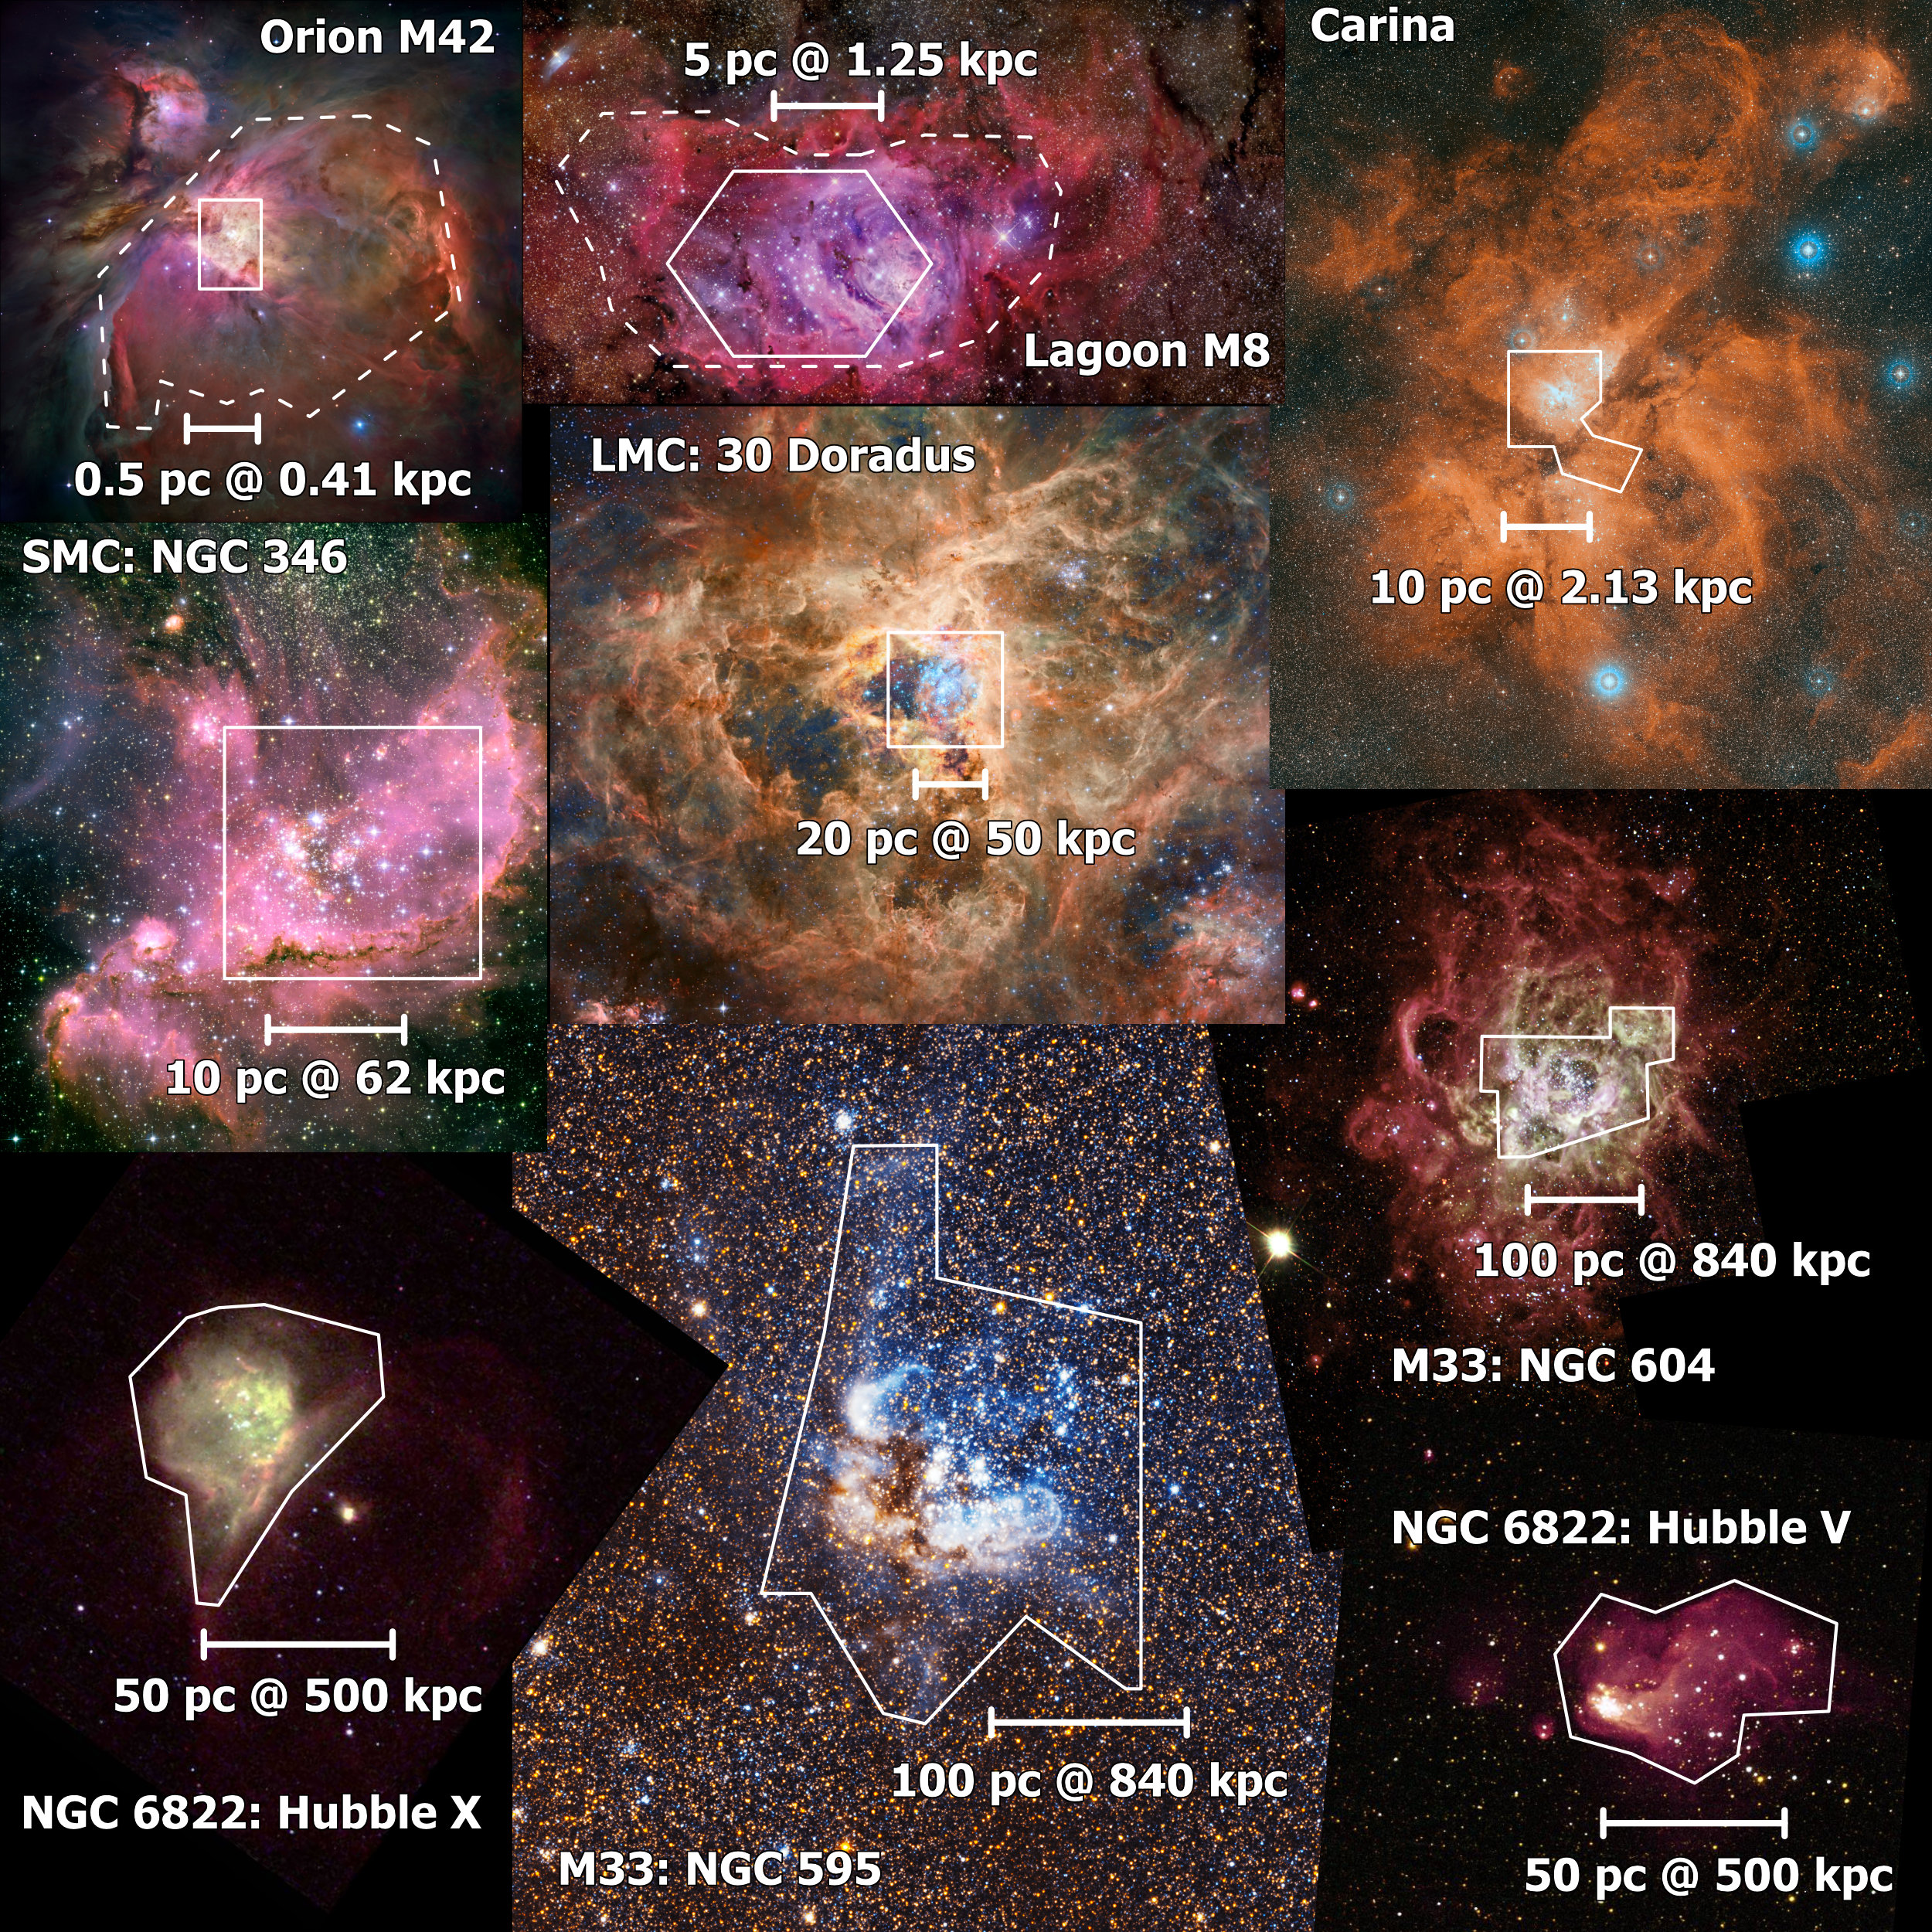
\includegraphics[width=\linewidth]{Figures/hii-region-mosaic}
  \caption{
    The sample of nine \hii{} regions employed in this study,
    arranged from top to bottom in order of distance.
    White shapes show the approximate extents of the
    emission line maps that we use for studying the ionized gas kinematics.
    Scale bars show the equivalent linear length scales at the distance to each region.
    For Orion, two fields are shown: the Extended Orion Nebula,
    sampled at a scale of \SI{0.1}{pc}, and the central Huygens region,
    sampled at a scale of \SI{0.004}{pc}.
    All images are combinations of optical narrow-band and wide-band filters.
    In most cases, red/orange/pink represents \ha{} or other emission lines
    emitted by the ionized gas,
    while blue/white represents continuum starlight from young high-mass stars.
    In some cases, green (for Hubble~X and NGC~604) or blue (for NGC~595)
    represents the [\ion{O}{3}] \Wav{5007} emission line.
    \textit{Image credits as follows.}
    \textbf{Orion Nebula}:
    \textit{HST} Treasury Program on the Orion Nebula Cluster \citep{Robberto:2013a}.
    \textbf{M8 Lagoon}: \href{https://www.cosmotography.com/index.html}{R.~Jay Gabany}.
    \textbf{Carina}: \href{https://www.eso.org/public/images/eso0905b}{
      ESO/Digitized Sky Survey~2, Davide De Martin}.
    \textbf{NGC~346}:
    NASA, ESA and A. Nota (ESA/STScI) \citep{Nota:2006x}.
    \textbf{30 Doradus}:
    \href{http://www.robgendlerastropics.com/Tarantula-HST-ESO.html}{
      Robert Gendler, Roberto Colombari,
      Hubble Legacy Archive, European Southern Observatories}.
    \textbf{Hubble~X}:
    \href{https://hubblesite.org/contents/media/images/2001/01/1012-Image.html}
    {C. R. O'Dell (Vanderbilt University),
      NASA and The Hubble Heritage Team (STScI/AURA)}.
    \textbf{Hubble~V}:
    \href{https://hubblesite.org/contents/media/images/2001/39/1126-Image.html}
    {C. R. O'Dell (Vanderbilt University)
      and L. Bianchi (Johns Hopkins University and Osservatorio Astronomico, Torinese, Italy),
      NASA, ESA, and The Hubble Heritage Team (STScI/AURA)}.
    \textbf{NGC~595}:
    \href{https://esahubble.org/images/heic1901c/}
    {NASA, ESA,
      and M. Durbin, J. Dalcanton, and B. F. Williams (University of Washington)}.
    \textbf{NGC~604}:
    \href{https://hubblesite.org/contents/media/images/2003/30/1423-Image.html}
    {NASA and The Hubble Heritage Team (AURA/STScI)}.
  }
  \label{fig:hii-regions}
\end{figure*}

\begin{figure*}
  \centering
  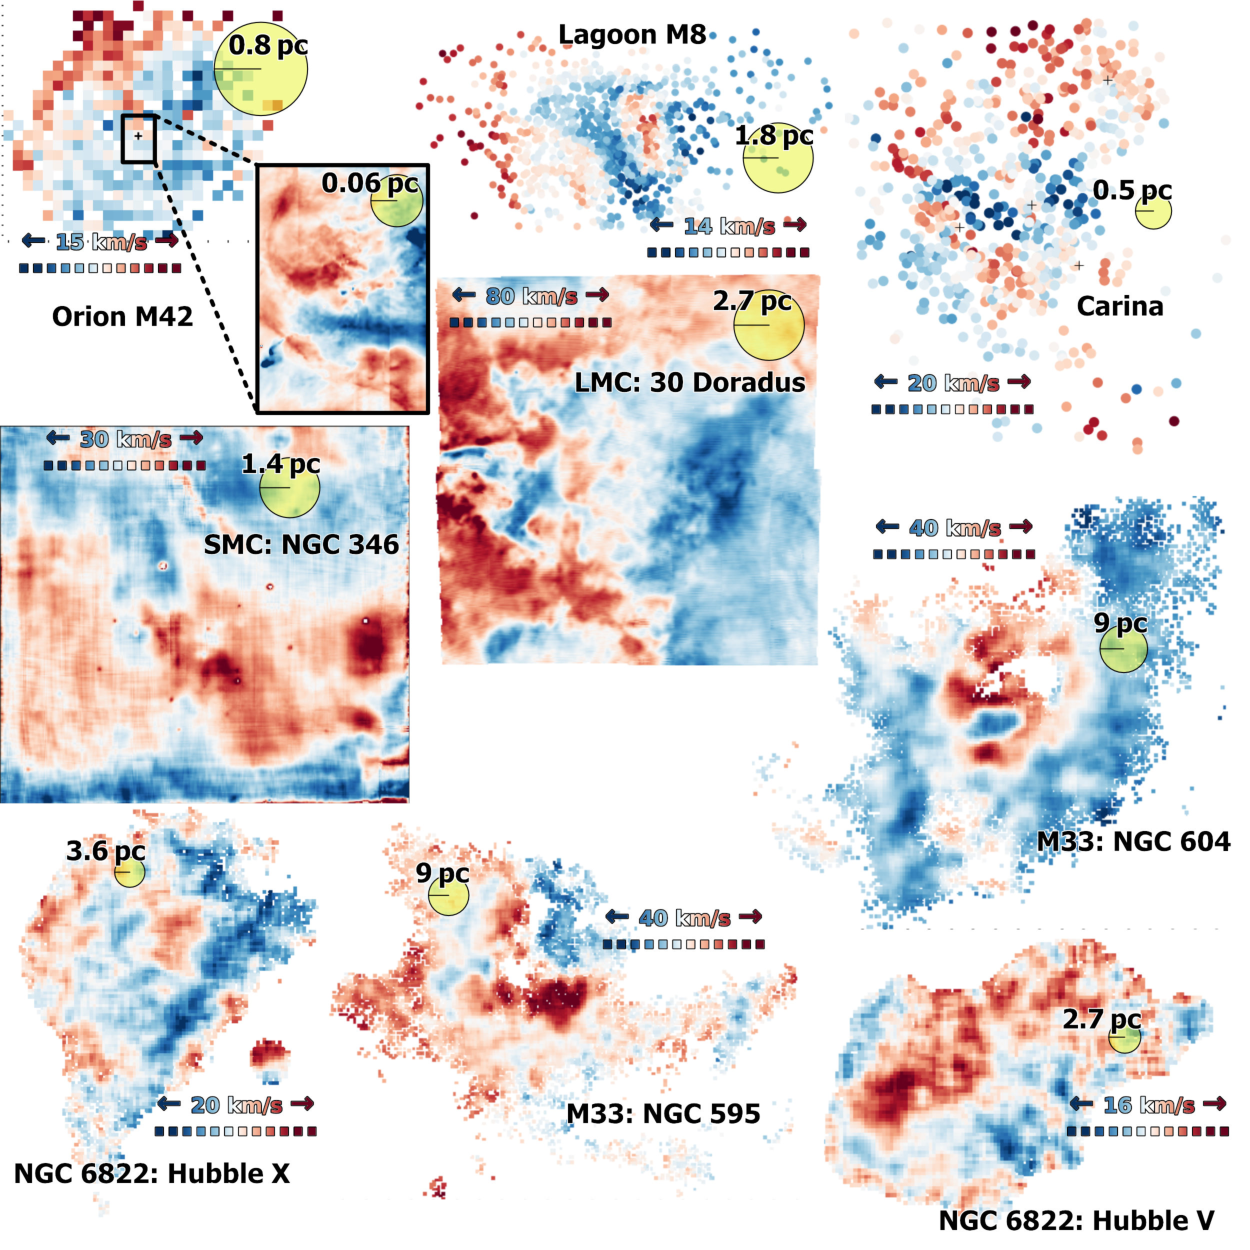
\includegraphics[width=\linewidth]{Figures/velocity-maps-mosaic}
  \caption{
    Maps of the mean \ha{} velocity for each of the regions in our sample.
    All velocities are relative to the systemic velocity of each region,
    with more negative velocities shown in blue and more positive velocities in red.
    The range of velocities is different for each region, as indicated on the individual maps.
    The correlation length of the velocity fluctuations in each region
    is shown as the radius of a yellow circle and labeled with its value in parsecs. 
  }
  \label{fig:velocity-maps}
\end{figure*}

Previous investigations of the centroid velocity structure function in \hii{} regions
have used a variety of methodologies, which makes it difficult to compare results
between different regions.  \citet{arthur2016turbulence} summarise historical results
for the Orion Nebula in their Table~5.
The most significant differences are seen when different emission line tracers are used,
but even when using the same line, there is some variance between different studies
in the derived values for both the velocity dispersion \(\sigma\pos\) and power-law slope \(m\).
It is therefore worthwhile to employ a uniform approach across a variety of different regions.
To that end, we have selected 9 \hii{} regions,
covering a broad range in size and luminosity,
for which good quality mapping of the \ha{} line exists in the literature
or in data archives.
Figure~\ref{fig:hii-regions} shows optical images of
each region in our sample
and Table~\ref{tab:regions-properties} lists their most important physical parameters.
The derived centroid \ha{} velocity maps are shown in Figure~\ref{fig:velocity-maps}.
Our sample includes three Milky Way regions
(at approximate distance of \num{0.5} to \SI{2}{kpc}),
two regions in the Magellanic Clouds (\num{50} to \SI{60}{kpc}),
and four regions in more distant galaxies of the Local Group
(\num{500} to \SI{800}{kpc}).
Further details of the observations and the sources themselves
are given in the following two sections.

\subsection{Spectroscopic datasets}
\label{sec:spectr-datas}

\newcommand\xx{\ensuremath{\boldsymbol{x}}}
Wherever possible, we calculate the centroid velocity \(V_c\)
directly as the normalized first velocity moment of the spectral line intensity profile
for each plane-of-sky position \(\xx\) on the nebula:
\(V_{c}(\xx) = M_1(\xx) / M_0(\xx)\).
The \(k\)th unnormalized moment \(M_k\) of the continuum-subtracted
spectral intensity profile \(I(v)\)
is defined as
\begin{equation}
  \label{eq:kth-moment}
  M_k = \int_{\Delta v} I(v) \, v^k \, dv
\end{equation}
where the Doppler velocity \(v\) is calculated according to
the \texttt{VOPT} convention
\citetext{Eq.~[32] of \citealt{Greisen:2006a}}:
\begin{equation}
  \label{eq:optical-velocity}
  v \equiv c\, (\lambda - \lambda_0) / \lambda_0 ,
\end{equation}
where \(\lambda\) is the observed wavelength,
\(\lambda_0\) is the rest wavelength, and \(c\) is the speed of light.
The spectral window \(\Delta v\) is chosen to be just large enough to include
the entire \ha{} emission line.
So long as the signal-to-noise is high enough,
this mean velocity can be calculated to a much higher precision
than the nominal velocity resolution of the spectrograph. 
In a few cases, as noted below, we are working with already reduced data,
which are provided in the form of Gaussian fits to the line profiles.
In the cases where multiple Gaussian components have been fitted,
we take the flux-weighted mean velocity of these components to be the centroid.

The observed RMS spectral line width \(\sigma'\) can likewise be found from
the second velocity moment as
\begin{equation}
  \label{eq:observed-sigma}
  \sigma'(\xx)^2  = [M_2(\xx) / M_0(\xx)] - V_{c}(\xx)^2 .
\end{equation}
However, many different broadening mechanisms contribute to this width,
including the finite spectral resolution \(\sigma_{\mathrm{ins}}\),
fine-structure splitting \(\sigma_{\mathrm{fs}}\),
and thermal Doppler broadening \(\sigma_{\mathrm{t}}\).
In the approximation that all these broadening mechanisms are independent
and described by Gaussian profiles, then the dispersion of
line-of-sight velocities due to bulk motions \(\sigma\los\) can be found
by subtracting these contributions in quadrature from the observed width:
\begin{equation}
  \label{eq:sigma-los}
  \sigma\los^2 = \sigma'^2 - \sigma_{\mathrm{ins}}^2 - \sigma_{\mathrm{fs}}^2 - \sigma_{\mathrm{t}}^2 .
\end{equation}
See sec~5.1 of \citet{Garcia-Diaz:2008a} for further details.

\subsubsection{Longslit echelle spectroscopy}
\label{sec:longsl-echelle-spect}

For the Orion Nebula, we use data obtained with the echelle spectrograph attached to the \SI{4}{m} telescope at Kitt Peak National Observatory (KPNO) initially published in
\citet{Doi:2004a}.
These observations cover a \(\SI{3}{arcmin} \times \SI{5}{arcmin}\) region of the
central (Huygens) part of the Orion Nebula.
The data consist of 96 North--South orientated \SI{300}{arcsec} slits,
uniformly spaced at \SI{2}{arcsec} intervals with a width of \SI{0.8}{arcsec}
with a velocity resolution of \SI{8}{km.s^{-1}}. 
For the centroid velocities, we use the intensity-weighted 
mean velocities calculated by \citet{Garcia-Diaz:2008a},
who used additional observations with East--West oriented slits
to refine the inter-slit velocity calibration. 
Unlike in the previous analysis of this dataset by \citet{arthur2016turbulence},
we do not mask out regions affected by known high-velocity outflows.
This decision was made for consistency with the analysis of more distant regions,
where such a masking out is not possible.

\subsubsection{Fabry-Pérot étalon}
\label{sec:fabry-perot-etalaon}

We use \cite{1987A&A...176..347H} observations to analyze the Extended Orion Nebula.
These observations were obtained using a 106 cm-Cassegrain telescope at Observatorium Hoher List. 
A Fabry-Pérot interferometer was used with a étalon separation of 0.5 mm. 
A number of fifteen interferograms have been taken with different pointing directions of the telescope's optical axis in the nebula with an exposure time between 10 and 40 minutes. 
The exposures are overlapped and fall into one square of a grid with a width of 1' centered at \(\theta^{1}\)Ori C.   

\subsubsection{FLAMES multi-fiber spectroscopy}
\label{sec:flames-multi-fiber}

Archival data from \citet{Damiani:2016a} and \citet{Damiani:2017b} are used
to study the Carina Nebula and Lagoon Nebula, respectively.
These were obtained as a by-product of a study of young stars in their respective regions
as part of the Gaia-ESO Spectroscopic Survey \citep{Gilmore:2012v, Randich:2013m}
using VLT/FLAMES with the GIRAFFE and UVES spectrographs \citep{2002Msngr.110....1P}.
The spectra are from multiple discrete fiber positions in each nebula
(866 positions in Carina; 1089 in the Lagoon),
visible as colored disks in Figure~\ref{fig:velocity-maps}.
The angular separation between fibers varies across the maps with
average nearest-neighbor distance of \SI{21 \pm 17}{arcsec}.
The spectral resolution ranges from  \SI{6}{km.s^{-1}} (UVES) to \SI{16}{km.s^{-1}} (GIRAFFE).
We do not have access to the individual spectra, but instead use the
Gaussian fits to the line profiles from \citep{Damiani:2016a, Damiani:2017b},
obtained from data tables downloaded from the CDS Vizier service.\footnote{%
  \url{https://doi.org//10.26093/cds/vizier.35910074} and
  \url{https://doi.org//10.26093/cds/vizier.36040135}.}
For the Lagoon, we use single-Gaussian fits, while for Carina we take the
flux-weighted mean of the blue and red component of two-Gaussian fits.


\subsubsection{MUSE integral field spectroscopy}
\label{sec:muse-integral-field}

For the Magellanic Cloud regions 30~Doradus and NGC~346 we use data obtained
with the MUSE spectrograph \citep{Bacon:2010a, Bacon:2014a} on the VLT.\@
Each exposure consists of a \(300 \times 300\) pixel spectral image with a plate scale
of \SI{0.2}{arcsec.pixel^{-1}} and a spectral resolution of \SI{110}{km.s^{-1}}
at \ha{}.
For 30~Doradus, four separate exposures are mosaicked to give a square field of
size \(\SI{2}{arcmin}\) \citep{Castro:2018a}. 
We use centroid velocities of single Gaussian fits to the \ha{} line.\footnote{%
  Data kindly provided by Norberto Castro Rodríguez, priv.~comm.
}
For NGC~346, we use a single field that was observed in 2016 as part of
ESO observing program 098.D-0211(A) (P.I. W.-R.~Hamann).
We obtained the pipeline-reduced data cubes from the ESO data archive\footnote{%
  \url{http://archive.eso.org/wdb/wdb/eso/eso_archive_main/query?prog_id=098.D-0211(A)}
}
and extracted the \ha{} profile using tools in the MPDAF python library.\footnote{
  \url{https://mpdaf.readthedocs.io/en/latest/}
} 

\subsubsection{TAURUS-II Fabry-Perot spectroscopy}
\label{sec:taurus-ii-fabry}

The archival data used in this work for the extragalactic giant regions, NGC 604, NGC 595, Hubble X and Hubble V was obtained with the Fabry Perot TAURUS-II instrument
\citep{Gordon:2000v}
on the \SI{4.2}{m} William Herschel Telescope (WHT) of
el Roque de los Muchachos Observatory (ORM) in La Palma, Spain
and was retrieved from the La Palma archive\footnote{\url{http://casu.ast.cam.ac.uk/casuadc/ingarch}}.
Each velocity image is \(256 \times 256\) pixels on the sky,
with a spatial scale of \SI{0.26}{arcsec.pixel^{-1}}
and a spectral resolution of \SI{40}{km.s^{-1}}.
The NGC~604 observations were previously reported and analyzed in
\citet{sabalisck1995supersonic}, \citet{Medina-Tanco:1997a} and \citet{Melnick:2021x}.

% \citet{sabalisck1995supersonic} mentioned the main aspects of the observations (1990 July 31).
% The two-dimensional imaging spectroscopy was captured using an IPCS-II detector and the 125 $\mu$m etalon.
% The cumulative integration time per frame is 36 s with a seeing value of 1''.
% The format of the data cube was of 256*256*100 with a spatial scale of 0.26 pixel$^{-1}$.
% Finally, the reduction and analysis was done with the packages TAUCAL y TAUFITS \citep{1992ASPC...25..445L}. The NGC 604 TAURUS-II observations were used by \citet{sabalisck1995supersonic}, \citet{tanco1997} and \citet{2019arXiv191203543M}.


\subsection{Physical properties of the sample regions. }
\label{sec:regions-milky-way}

\begin{table}
\begin{center}\caption{Summary of properties of our \hii{} region sample. Sizes taken from Table 2 of \citet{1984ApJ...287..116K}. Reference from the other properties are mentioned in the text.}
\begin{tabular}{cCCCC}\toprule
\hii{}    &  \text{Distance,}\ d& \text{Size,}\ S & \log L(\ha) &  \langle \sigma\los \rangle \\
  Region    &  [\si{kpc}]          &  [\si{pc}]    &  [\si{erg.s^{-1}}]            &    [\si{km.s^{-1}}]  \\ 
\midrule
Orion     & 0.436 \pm 0.02  & 5 \pm 0.5    &    37.18       &   6 \pm 1      \\
Lagoon    & 1.25 \pm 0.12   & 25 \pm 2.5      &    37.47    &   13.6 \pm 0.8    \\
Carina    & 2.35 \pm 0.05   & 200 \pm 20      &    38.54    &   22.4 \pm 2.7    \\
30 Dor    & 50.0 \pm 0.2    & 370 \pm 37    &    39.46    &   31.7     \\
NGC 346   & 62 \pm 1        & 220 \pm 22      &    38.77    &   10.1     \\
Hubble X  & 490 \pm 40      & 160 \pm 16      &    38.21    &   13.4     \\
Hubble V  & 490 \pm 40      & 130 \pm 13      &    38.3     &   12.3     \\
NGC 595   & 820 \pm 30      & 400 \pm 40      &    38.95    &   18.3 \pm 5.7     \\
NGC 604   & 820 \pm 30      & 400 \pm 40      &    39.42    &   16.2 \pm 7.7     \\
\bottomrule
\end{tabular}\label{tab:regions-properties}
\end{center}
\end{table} 

\subsubsection{Orion Nebula}
\label{sec:orion-nebula}

The Orion Nebula (M42) is the prototype of a galactic HII region located at a distance of 440 pc \citetext{\SI{1}{\arcsecond} = \SI{0.001}{pc} ; \citealp{2008AJ....136.1566O}}.
The O7 V star \(\theta^{1}\) Ori C is the most luminous and hottest star \citep{2006A&A...448..351S} with an ionizing flux \(Q_0\) of  \SI{e49.12}{photons.s^{-1}}. 
With other 3 B-type stars they form the Trapezium cluster.
The bright region that surrounds these massive ionizing stars is called the the Huygens region (Orion core henceforth).
In the southwest direction of the Huygens region there is a drop in the brightness as one approach a much larger region called Extended Orion Nebula \citetext{EON henceforth;  \citealp{2008Sci...319..309G}}
The position of Orion near the side of the Orion Molecular Cloud (OMC-1) make it an ongoing star formation with a large population of young star, some of which are the sources of stellar jets and Herbig-Haro objects \citep{1993ApJ...410..696O}.
Its physical properties and kinematics, along its stellar population are documented in \citet{2001ARA&A..39...99O}.

\subsubsection{Lagoon Nebula}
\label{sec:lagoon-nebula}

The Lagoon Nebula (M8, NGC6523) is located at a distance of 1 250 pc \citetext{\SI{1}{\arcsecond} = \SI{0.006}{pc} ; \citealp{2005A&A...430..941P}}.
It has a luminosity in \ha{} of \SI{e37.47}{erg.s^{-1}}\citep{1984ApJ...287..116K}.
It contains the young stellar cluster NGC6530 and the region is illuminated by different massive stars of spectral types O and B, the hottest being 9 Sgr, type O4V \citep{Damiani:2017b}.
Optically, the brightest part of the nebula is called 'Hourglass nebula' which surrounds and obscures the O7 star Herschel 36 \citep{1986AJ.....91..870W}. 
The velocity field shows several expanding shells, related to the stellar population, and the massive protostar M8East-IR \citep{1984ApJ...278..170S} indicating that recent star formation. 
A blueshifted, neutral layer is also in very good agreement with predictions of champagne-flow models of blister HII regions \citep{Damiani:2017b}. 
The properties of the nebula are reviewed by \citet{2008hsf2.book..533T}.

\subsubsection{Carina Nebula}
\label{sec:carina-nebula}

The Carina nebula is a large star-forming complex located at a distance of 2 350 pc \citetext{\SI{1}{\arcsecond} = \SI{0.01}{pc} ; \citealp{2006ApJ...644.1151S}}.
Using the \ha{} luminosity as a diagnostic of the ionizing flux \(Q_0\) \citet{2007MNRAS.379.1279S} measured a value of \SI{e50.47}{photons.s^{-1}}.
Young clusters like Trumpler 14 and 16, and Collinder 228 form the Car OB1 association, one of the largest OB associations on the Galaxy.
This OB association has more than 65 stars earlier than B0, and several Wolf-Rayet (WR) stars.
The most luminous star is the blue variable $\eta$ Car.
As a star formation region, it presents several phenomena related with young stars as evaporating protoplanetary discs, erosion of large dust pillars and the triggering of a second generation of embedded stars and Herbig-Haro objects, to mention some \citetext{see \citealp{2008hsf2.book..138S} and reference therein}. 
This region can be consider as a bridge between the detailed star-formation regions like Orion, and much more distant regions like 30 Doradus.
 
\subsubsection{30 Doradus}
\label{sec:30-doradus}

The 30 Doradus (Tarantula Nebula) nebula is located at a distance of 49.9 kpc \citetext{\SI{1}{\arcsecond} = \SI{0.24}{pc} ; \citealp{2013Natur.495...76P}}.
It is a luminous star-forming region in the LMC (Large Magellanic Cloud) and is the most luminous complex in the Local Group \citep{1984ApJ...287..116K}.
The central ionized region spans for 40 pc and host the massive, dense star cluster R136 %\citep{1991IAUS..148..145W}. %Note: check the bibliographic format
The ionizing output \(Q_0\) of R136 is \SI{e51.4}{photons.s^{-1}} \citep{2020MNRAS.499.1918B}.
It host the active star forming region NGC 2070 \citep{2013AJ....145...98W} where the star-formation rate has recently peaked \citep{2015ApJ...811...76C}. 
NGC 2070 host a population of OB and WR stars \citep{2011A&A...530A.108E}.
This nebula is commonly used as a comparison for extragalactic star-forming regions.

\subsubsection{NGC 346}
\label{sec:ngc-346}

NGC 346 is the most active star-formation region in the SMC (Small Magellanic Cloud) located at a distance of 62 kpc \citetext{\SI{1}{\arcsecond} = \SI{0.30}{pc} ; \citealp{2001ApJ...562..303D}}. 
It has more than 30 O stars that ionize N66, the largest HII region \citep{2011ApJ...740...10D}.
N66 has an \ha{} luminosity of \SI{e38.77}{erg.s^{-1}}, almost 60 times higher compared to the Orion Nebula \citep{2010A&A...517A..39H,1984ApJ...287..116K}.
\citet{2008ApJ...688.1050G} propose an expanding HII region or bubble blown by the winds of the massive progenitor as a mechanism that shapes the recent star formation in this region, in addition to the photoionizing process of the OB stars. 
This mechanism is similar to shell-like HII regions, with a central cluster in a cavity, and with ongoing star formation triggered around their periphery.
Using a Gaussian single-component \citet{2003ApJ...586.1179D} find a corrected FWHM bulk turbulence of \SI{23.8}{km.s^{-1}}. 

\subsubsection{Hubble X and Hubble V in NGC 6822}
\label{sec:6822-hubble}
%Note to me: incomplete section. Find more regions info and finish asap.
The irregular dwarf galaxy, NGC 6822, is located at a distance of 500 kpc \citetext{\SI{1}{\arcsecond} = \SI{2.42}{pc} ; \citealp{2012A&A...540A.135S}} and the brightest HII regions are Hubble X and Hubble V (HX and HV hereafter). %(1'' = 2.4 pc)
%HV has a characteristic length of 100 pc and HX has a characteristic length of 140 pc \citep{1999PASP..111.1382O}.
Luminosity \ha{} for HV is \SI{e38.3}{erg.s^{-1}} and for HX is \SI{e38.21}{erg.s^{-1}} \citep{2002MNRAS.329..481B}.
Two recognized OB associations are identified within these HII regions \citep{1991ApJ...379..621H,1992AJ....104.1374W}.
HV is located near 'Hodge OB 8' and HX is located near 'Hodge OB13'  \citep{1999PASP..111.1382O}.

%HV has a luminosity at its core of in L$_{H_\alpha}$ = 1 $\times$ 10$^{49}$ H$\alpha$ photons s$^{-1}$ 
%HX has a luminosity at its core of in L$_{H_\alpha}$ = 2.4 $\times$ 10$^{49}$ H$\alpha$ photons s$^{-1}$ \citep{1999PASP..111.1382O}.

\subsubsection{NGC~595 and NGC~604 in M33}
\label{sec:m33-ngc}

M33 is the third largest galaxy in the Local Group located at the distance of 840 kpc \citetext{\SI{1}{\arcsecond} = \SI{4.07}{pc} ; \citealp{2015KamKinematics}} and is of morphological type SA(s)cd.
The two brightest HII regions in the galaxy are NGC 604 and NGC 595.

NGC 604 is the second brightest \hii{} region in the Local Group after 30~Dor in the Large Magellanic Cloud and is forty times larger ($\sim $ 400 pc) and 6,000 times brighter than Orion in our Milky Way galaxy.
It is the brightest giant \hii{} region in the M33 galaxy and is visually dominated by a big loop, big shells and different size filaments.
It has a luminosity in \ha{} of \SI{e39.42}{erg.s^{-1}} \citep{2002MNRAS.329..481B}.
Using photometry from the HST \citet{1996ApJ...456..174H} identified that the stars are separated into a primary cluster within NGC 604, and a secondary to the north of the region.
In the primary there are \(\sim\)200 OB stars, candidate to red supergiants (RSGs) and the presence of WR stars.
For the northern cluster they find eight luminous stars and no evolved massive stars.
More Recently, \citet{2011MNRAS.411..235E} studied 10 WR stars and propose at least 4 RSGs candidates.
\citet{2012AJ....143...43F} focused on the massive young stellar objects (MYSOs).
The average ages for the stars, was determined to be from  \num{3} to \SI{5}{Myr} \citep{1996ApJ...456..174H} and with the RSGs as an older population have an age of 12.4\(\pm\)2.1 Myr \citep{2011MNRAS.411..235E}.
This suggest that two episodes of star formation, at least, have taken place in the GEHR.

% and in L$_{X}$=9.3$\times$ 10$^{35}$ erg s$^{-1}$ \citep{2008ApJ...685..919T}.
%\citet{2012ApJ...761....3M} derive an average age of 4$\pm$1 Myr and a total stellar mass of 1.6$^{+1.6}_{-1.0} \times$ 10$^{5}$M$_{\odot}$ for the region.

NGC 595 is the second brightest giant HII region in the M33 galaxy and has an \ha{} shell morphology that is related to the stellar winds of the several massive stars located in its interior.
It has a luminosity in \ha{} of \SI{e38.95}{erg.s^{-1}}\citep{2002MNRAS.329..481B}.
\citet{1993AJ....105.1400D} use optical photometry to propose 11 WR stars. 
Using HST/WFPC-2 images \citet{1996AJ....111.1128M} found approximately 250 stars of the OB type, 13 Supergiants and 10 WR, confirming previous candidates.
They derived and age of 4.5\(\pm\)1.0 Myr consistent with \citet{1993AJ....105.1400D}.
\citet{2010MNRAS.402.1635R} used Integral Field Spectroscopy (IFS) to present a resolved study of the physical properties of the ionized gas and the ionized structure.
They also confirm the presence of previous cataloged WR stars and detect new candidates, and propose classical emission-line ratios as metallicity calibrators.
\citet{lagrois2011} present a kinematic study of the regions using optical emission lines and and radio 21 cm line observations.
They proposed Champagne flows at the periphery of the molecular cloud leading to accelerated ionized material.

%%%%%%%%%%%%%%%%%%%%%%%%%%%%%%%%%%%%%%%%%%%%%%%%%%%%%%%%%%%%%%%%%%%%%%%%%%%%%%%%%%%%%%%%%%%%%%%%%%%%
%%%%%%%%%%%%%%%%%%%%%%%%%%%%%%%%%%%%%%%%%%%%%%%%%%%%%%%%%%%%%%%%%%%%%%%%%%%%%%%%%%%%%%%%%%%%%%%%%%%%%%%

\section{Plane-of-sky velocity fluctuations}\label{sec:met}

Figure~\ref{fig:velocity-maps} shows maps of the \ha{} centroid velocity
\(V_c\) for each \hii{} region in our sample,
calculated as described above in section~\ref{sec:spectr-datas}
and after subtracting the mean systemic velocity,
\(\left\langle V_c\right\rangle\) in each case.
% The color scheme ranges from the most negative velocities in blue
% to the most positive velocities in red,
% but the amplitude of the velocity fluctuations differs considerably between regions,
% as indicated by the color scale bar on each map,
% ranging from \SI{\pm 7}{km.s^{-1}} for the Lagoon
% up to  \SI{\pm 40}{km.s^{-1}} for 30~Doradus.
The overall amplitude of the plane-of-sky
velocity fluctuations can be characterized by a dispersion,
\(\sigma\pos\), defined as:
\begin{equation}
  \label{eq:sig-pos}
  \sigma^2\pos =
  \left\langle 
  \bigl[ V_c (\xx_i) -\langle V_ c\rangle  \bigr]^2
  \right \rangle ,
\end{equation}
where the average is performed over all observed points \(i\)
in a given map.
Note that \(\sigma\pos\) is also the RMS width of
the probability density function (PDF) of \(V_c\).
This PDF for each region is shown in Figure~\ref{fig:hist}
on a common velocity scale and arranged in order of decreasing \(\sigma\pos\).
It can be seen that the amplitude of the
velocity fluctuations varies considerably between regions,
with \(\sigma\pos\) in 30~Dor being more than 5 times higher than in 
nearby regions such as Orion.

All of the PDFs are significantly non-Gaussian
and many show evidence of a multi-modal structure.
Some, such as Orion core and Hubble~V, show a single dominant velocity component,
but most show several distinct peaks,
as many as four in the case of Carina.
There is no clear tendency for the number of identifiable velocity components
to increase with increasing velocity dispersion.
Instead, both the widths of the individual peaks and the separation between them
seem to increase in tandem.
For most regions the PDFs are approximately symmetrical,
but two regions show significant skewness:
Orion~core has a smooth asymmetrical tail towards the blue,
whereas NGC~346 has one towards the red.

\begin{figure*}
 \centering
 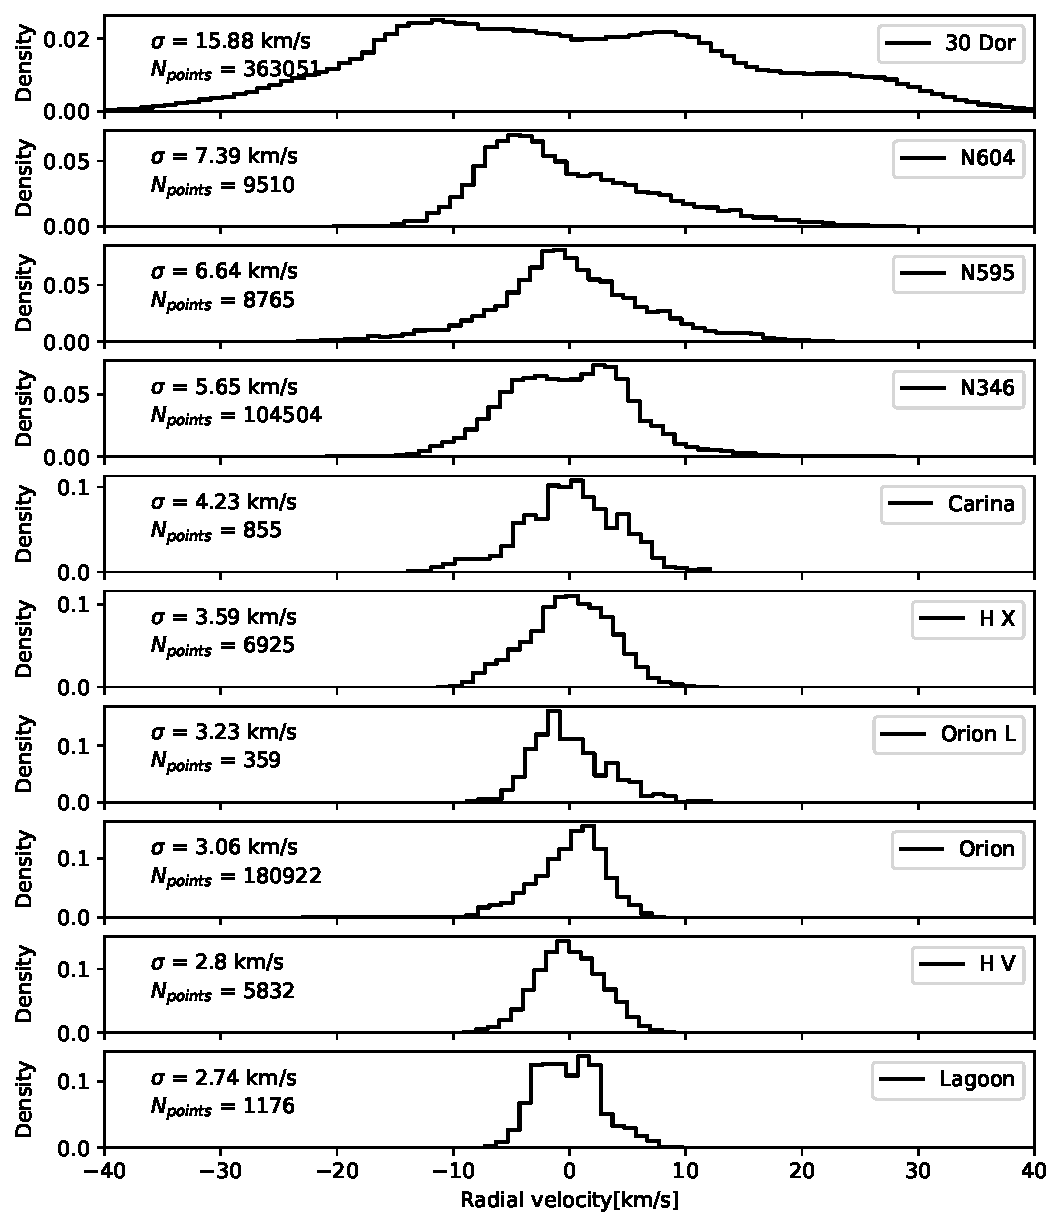
\includegraphics[width=5in]{Figures/Hist}\par
 \caption{
   Histograms of the plane-of-sky variation in the \ha{} centroid velocities.
   Each panel shows the fraction of the observed spatial points
   (pixels or fiber positions)
   with a given velocity offset from the mean systemic velocity of each region.
   The RMS width \(\sigma\pos\) of each distribution is marked,
   as is the number of spatial points.
   The bin width is \SI{1}{km.s^{-1}} and the regions are arranged
   in order of decreasing \(\sigma\pos\).
 }
 \label{fig:hist}
\end{figure*}


\subsection{The second-order structure function}
\label{sec:second-order-struct}
% One of the fundamental properties of turbulent clouds must be spatial fluctuations in velocity and density.                                     
% These fluctuations are observed as projected spatial fluctuations in the average line-of-sight velocity and integrated column density.
% It is possible to describe the statistical properties of these fluctuations if they are assumed as a product of a stochastic field \citep{1984ApJ...277..556S}. 
% This previous assumption give us the ability to apply statistical tools to the velocity field and the analysis of the velocity pattern is reduced to the calculation of the averages and correlations.

In order to probe the dependence of the velocity fluctuations
on spatial scale,
the primary tool that we employ is
the second order structure function of differences in velocity centroids,
$B(r)$, which is a function of the scalar separation or lag, \(r\),
between two points on the plane of the sky:
%
\newcommand\Abs[1]{\vert #1\vert}
\begin{equation}\label{eq:Br}
  B(r) = \left\langle 
  \bigl[
  V_{c}(\xx_j) - V_{c}(\xx_i)
  \bigr]^{2} \right \rangle_{\Abs{\xx_j - \xx_i\!} \ \approx \ r} \ .
\end{equation}
The averaging is performed over all pairs of points
\((i, j)\)
whose scalar separation \(\Abs{\xx_j - \xx_i}\) is close to \(r\),
irrespective of the orientation of the separation vector.
In practice, we achieve this by binning the separations with a constant
logarithmic width of \SI{0.15}{dex}.

We will also employ the related quantity of the
normalized spatial autocovariance or autocorrelation function:
\begin{equation}
  \label{eq:autocovar}
  C(r) = \frac{1}{\sigma^2\pos}\left\langle 
  \bigl[
  V_{c}(\xx_j) \  V_{c}(\xx_i)
  \bigr]^{2} \right \rangle_{\Abs{\xx_j - \xx_i\!} \ \approx \ r} \ .
\end{equation}
If the fluctuations are perfectly spatially homogeneous, then the
two quantities are related \citep{1984ApJ...277..556S} as
\begin{equation}\label{eq:functional}
  B(r) = 2\sigma^2\pos \bigl[   1 - C(r)\bigr] .
\end{equation}
In less ideal situations, then \(B(r)\) is to be preferred since it is
relatively unaffected by non-stationary effects
such as large-scale linear gradients 
\citep{1984ApJ...277..556S}.
Nonetheless, \(C(r)\) is more amenable to heuristic reasoning in some cases,
which we will take advantage of below.


\subsection{A heuristic model for the structure function}
\label{sec:methods-apply}

A common property of homogeneous fluctuating velocity fields is that neighboring points tend to have similar velocities
(\(C(r) \approx 1\) for small \(r\)),
whereas points that are far apart may have very different velocities
(\(C(r) \ll 1\) for large \(r\)).
The value of the separation that corresponds to
the transition between these two regimes
is called the correlation length, \(r_0\).
In the simplest case,
two points separated by \(r \gg r_0\) have totally uncorrelated velocities
in the sense that knowledge of the velocity at the first point is of
no help in predicting the velocity at the second point.
At scales smaller than \(r_0\), the fluctuations often show a power-law behavior.

In order to capture these two behaviors,
We therefore propose the following idealized 2-parameter model
for the autocorrelation function:
%
\begin{equation}\label{eq:new-correlation-form}
  C(r;\ r_0, m) = \exp \left[ -(\ln 2) \left( \frac{r}{r_0} \right)^m \right].
\end{equation}
%
in which \(r_{0}\)\ is the correlation length (see above)
and \(m\) is the power-law slope at small scales.
This is constructed so that \(C(r) = 1/2\) at \(r = r_0\),
while the exponential form ensures that \(C(r)\) rapidly approaches zero
for larger separations.
We use equation \eqref{eq:functional} to determine the structure function
from this model autocorrelation function.
The resultant model structure function has the following properties:
\begin{enumerate}[1.]
 \item Small scales: \(B(r) \propto r^m\) for \(r \ll r_0\);
 \item Correlation scale: \(B(r_0) = \sigma^2\);
 \item Large scales: \(B(r) \to 2 \sigma^2\) for \(r \gg r_0\).
\end{enumerate}
In a previous paper, we used a different functional form
\citetext{See Fig.~13 of \citealp{arthur2016turbulence}}:
\(C(r) = 1/[1+(r/r_{0})^{m}]\), as proposed in \citet{1984ApJ...277..556S},
which behaves identically to equation~\eqref{eq:new-correlation-form}
in the first two regimes, but is more gradual in its approach
to the large-scale asymptote of \(2 \sigma^2\).
However, we find that equation~\eqref{eq:new-correlation-form}
provides a much improved fit to the observed structure functions
of our sample regions (see following section). 


% The term \(r_{0}\)\ is the correlation length where the value of separation \(r\) reach the value of \(\sigma^2\) in the structure function and $m$ is the power-law index that fits the inertial scale.
% In an idealized case at scales larger than \(r_{0}\)\ the structure function flattens as it tends towards the asymptotic value of 2\(\sigma^2\) \citep{arthur2016turbulence}.
% This substitutes the previously \(C(r) = 1/[1+(r/r_{0})^{m}]\) from \citet{1966igd..book.....K} and
% \citet{1984ApJ...277..556S}.

\subsubsection{Effects of observational limitations}
\label{sec:effect-observ-limit}

We also take into account in the new functional observational constraints like the seeing and observational box size (see Appendix~\ref{sec:degr-struct-funct} for details). 

The seeing becomes important at small scales and it is known that has an effect giving a more pronounced stepping in the structure function.
The model proposed to describe the seeing at small scales is:
%
\begin{equation}\label{eq:ffs}
   S(r; s_0, r_0) = \frac{
    e^{-s_0 / r_0}
  }{
    1+(2s_0 / r)^{2 / 3}
  }
\end{equation}

The model that consider the effect of the observational box size is:

\begin{equation}\label{eq:ffb}
% \beta(r_0) = 1 - exp[\frac{L_{box}}{3.6r_0}] 
  \beta(L,r_0) = 1 - \exp \left[ \frac{-L} {3.6 r_0} \right] 
\end{equation}
%
where the \(L\) value is the diagonal length of the observational box.

Considering the previous models we obtain the final form of our proposed structure function functional:
%
\begin{equation}\label{eq:sf-functional}
B_{\text{func}}(r) = B(r; \beta r_0, \beta \sigma^2,m) \times S(r; s_0, r_0) + B_{\text{noise}}
\end{equation}
%
where the term \( B_{\text{noise}}\) is a correction factor that considers the instrument noise at small scales.
This noise would have the effect of flattening the structure function by removing the effects of the fluctuations which would be interpreted as an uncorrelated field. 

The results obtained with equation \ref{eq:Br} are use in a non-linear least-squares fit with the equation \ref{eq:sf-functional} used as an objective function.
For this purpose we use the \textit{python} package \textit{lmfit} \citep{newville_matthew_2014_11813} where the equation \ref{eq:Br} and \ref{eq:sf-functional} are use in a chi-square statistic defined as:
%
%\begin{equation}\label{eq:chi}
%  \chi^2 = \sum_i ^N \frac{[y_i^{\text{measure}}-y_i^{\text{model}} (\boldsymbol{v})]^2}{\epsilon_i ^2}
%\end{equation}
%
%
\begin{equation}\label{eq:chi}
  \chi^2 = \sum_i ^N \frac{[B(r)-B_{\text{func}}(r;r_0, \sigma^2\pos, m, s_0, B_{\text{noise}})]^2}{\varepsilon_i ^2}
\end{equation}
%
which calculate a value \(\chi\) to be minimized scaled by the inverse of the uncertainty \(\varepsilon\) in the data.
The minimization procedure use the method \textit{emcee} \citep{2013PASP..125..306F} which is a \textit{python} implementation of the affine-invariant ensemble sampler for Markov chain Monte Carlo (MCMC) by \citet{2010CAMCS...5...65G}.  
The turbulent parameters \(r_{0}\)\ , \(\sigma^2\pos\) and \(m\), and the observational constraints \(s_0\) and \( B_{\text{noise}}\) are the set of variables in the model to be optimized in the fit.
Using these procedure we obtain posteriors for the structure function.

In this way we want to avoid one fundamental problem in the interpretation of the structure function. 
The slope in the majority of previous studies and hence, the correlation length, is obtained without a formal procedure. 
The traditional way to find the correlation length it is to determine a particular range of ascending values in the structure function. 
If this increase in values is stopped or reversed it is commonly assumed that one particular inertial range has been found. 
In some cases this procedure keeps going up to large scales, giving two or more inertial regimes leading to an erroneous interpretation of multiple inertial scales.

\subsubsection{Additional effects omitted from the model structure function}
\label{sec:limit-model-struct}

For separations that are comparable to the diameter \(D\) of the \hii{} region,
then the supposition of homogeneity may break down.
For instance, if the amplitude of the velocity fluctuations is higher
in the core of the region than in the outskirts,
then the autocorrelation function will be U-shaped
since all separations with \(r > D/2\) must be between two points in the outskirts,
which will tend to be relatively well correlated simply because both velocities
will be close to the mean.
This yields a corresponding downturn in the structure function at the largest scales.

Another example is if there were a periodic velocity fluctuation,
with spatial wavelength \(\lambda\),
then the autocorrelation function would become negative for \(r \approx \lambda/2, 3 \lambda / 2, \dots\),
which yields periodic peaks in the structure function.
Neither of these effects can be captured by our model structure function,
which assumes that the autocorrelation is strictly positive
and monotonically decreasing with \(r\).

At the very smallest scales, the autocorrelation function is predicted to
scale quadratically with \(r\)

\section{Results}\label{sec:results}

We present our second-order structure results plotted against separation in parsecs and the posteriors of the parameters used in the analysis.

\subsection{HII regions second-order structure functions and turbulent parameters}

Figures \ref{fig:strucfunc-fit-A}-\ref{fig:strucfunc-fit-D} left panels show in solid and open blue circles the observational structure function that we compute using equation \ref{eq:Br} on the \ha{} velocity fields of Fig. \ref{fig:velocity-maps}. The solid circles indicate the range use in the non-linear regression analysis (see section~\ref{sec:methods-apply}), while the open circles are the points of the structure function that where left out.
This was done to enhance the possibilities of a convergence since the structure function values at large separations are to follow the 2\(\sigma^2\) value according to theory.
The light shaded areas in the plots show where the separation \(r\) is above half of the box size \(L\), which is indicated with a vertical dotted line.

The green dashed line indicate the mean samples posterior of the model structure function without instrumental effects using equation \ref{eq:functional} and \ref{eq:new-correlation-form}.
The Figures also show in yellow solid line the mean of samples posterior using equation \ref{eq:sf-functional}.
The vertical dashed line indicates the correlation length value \(r_0\) and the horizontal dashed line indicates the true variance of the velocity fields, \(\sigma^2\).
The vertical and horizontal dotted lines shows the value of the observational considerations, the seeing, \(s_0\) and the value of the noise, \(B_{\text{noise}}\), respectively.
For the dashed and dotted lines the overlapping translucent boxes indicate the spread of values up to 2-sigma (dark shaded area) and 3-sigma (light shaded area) obtained after the analysis described in section~\ref{sec:methods-apply}.

Figures \ref{fig:strucfunc-fit-A}-\ref{fig:strucfunc-fit-D} right panels show the corner plots \citep{2017ascl.soft02002F} of the turbulent parameters and observational constraints. 
These plots shows the one and two dimensional projections of the posterior probability distributions of the parameters used in equation \ref{eq:chi}.
They also show the marginalized distribution for each parameter independently in the histograms along the diagonal and then the marginalized two dimensional distributions in the other panels making possible to visualize all of the covariances between parameters \citep{2017ascl.soft02002F}.
The contours in the plots reflect the 95\(\%\), 99\(\%\), 99.5\(\%\) and 99.9\(\%\) confidence intervals.

The results shown on left panels on Figures \ref{fig:strucfunc-fit-A}-\ref{fig:strucfunc-fit-D} show a typical second-order structure function pattern, where there is a series of ascending values of  the structure function that tends to stabilize around the 2\(\sigma^2\) value, indicating a loss in the correlations at large separations. 
The Carina nebula and Hubble X follow this behavior.

For astronomical observations it is thought that the values at large separations not following the previous pattern reflects movements that are not related to the ionized gas random motions.
It is known that HII regions are created on the edge of molecular clouds, so they will reach a blister or champagne phase, introducing large-scale gradients \citep{Mivi1995}. 
Also there is the expansion or rotation of each region.

A more common pattern for structure functions of HII regions looks like a 'hook' where at large separations the structure function values start decreasing.
This behavior is shown in the Orion core, 30 Doradus, Hubble V, NGC 595 and the EON.
Less common is the behavior where at large separations there are also a series of ascending values in the structure function, like the Lagoon nebula or NGC 346, or a periodic behavior like NGC 604.

Table \ref{tab:Res} presents the turbulent parameters results along the obtained observational constraints.

The second column correspond to the true variance \(\sigma^2\pos\) of the velocity field.
For all regions except for Carina, Lagoon and the EON there is an increase in this value.
For 30 Doradus, which has the highest value, \(\sigma\) goes from \SI{16}{km.s^{-1}} to  \SI{19}{km.s^{-1}}.
This is two times higher than NGC 604 that has a change of \SI{7}{km.s^{-1}} to \SI{9}{km.s^{-1}}, followed by NGC 595 with \SI{6.6}{km.s^{-1}} to \SI{7.5}{km.s^{-1}}.
NGC 346 is next with a value of \SI{6}{km.s^{-1}} which is close to the value of the centroid velocities.
Carina presents a value of \SI{4.2}{km.s^{-1}} which is the same as the velocity sample.
The Orion core has a change from \SI{3}{km.s^{-1}} to \SI{4}{km.s^{-1}}.
Hubble X has a value of \SI{3.9}{km.s^{-1}} which is very close with respect the \SI{3.6}{km.s^{-1}} value of the velocity field.
The value for Hubble V increase from \SI{2.8}{km.s^{-1}} to \SI{3.3}{km.s^{-1}}.
Lagoon presents a value of \SI{2.6}{km.s^{-1}} and the EON value decrease from \SI{3.2}{km.s^{-1}} to \SI{2.2}{km.s^{-1}}.
The \(B_{\text{noise}}\) value is shown in the third column which would be the minimum squared velocity difference that could be measure by the instrument.

The third column in Table \ref{tab:Res} shows the seeing value in parsecs, \(s_0\), which represent the minimum value of the separation which would valid for the observed structure function. 
The forth column shows the correlation value \(r_0\) in parsecs.
The \(r_0\) range covered in our results for the sample goes from 0.09 to 12 pc.
The fifth column indicates the size of each observational box in parsecs.
The index \(m\) is shown in the last column and the range covered by the power-law index in our HII region sample goes from 0.7 to 1.5.
The implications of these results is further developed on the next section.

\begin{figure*}
  \centering
  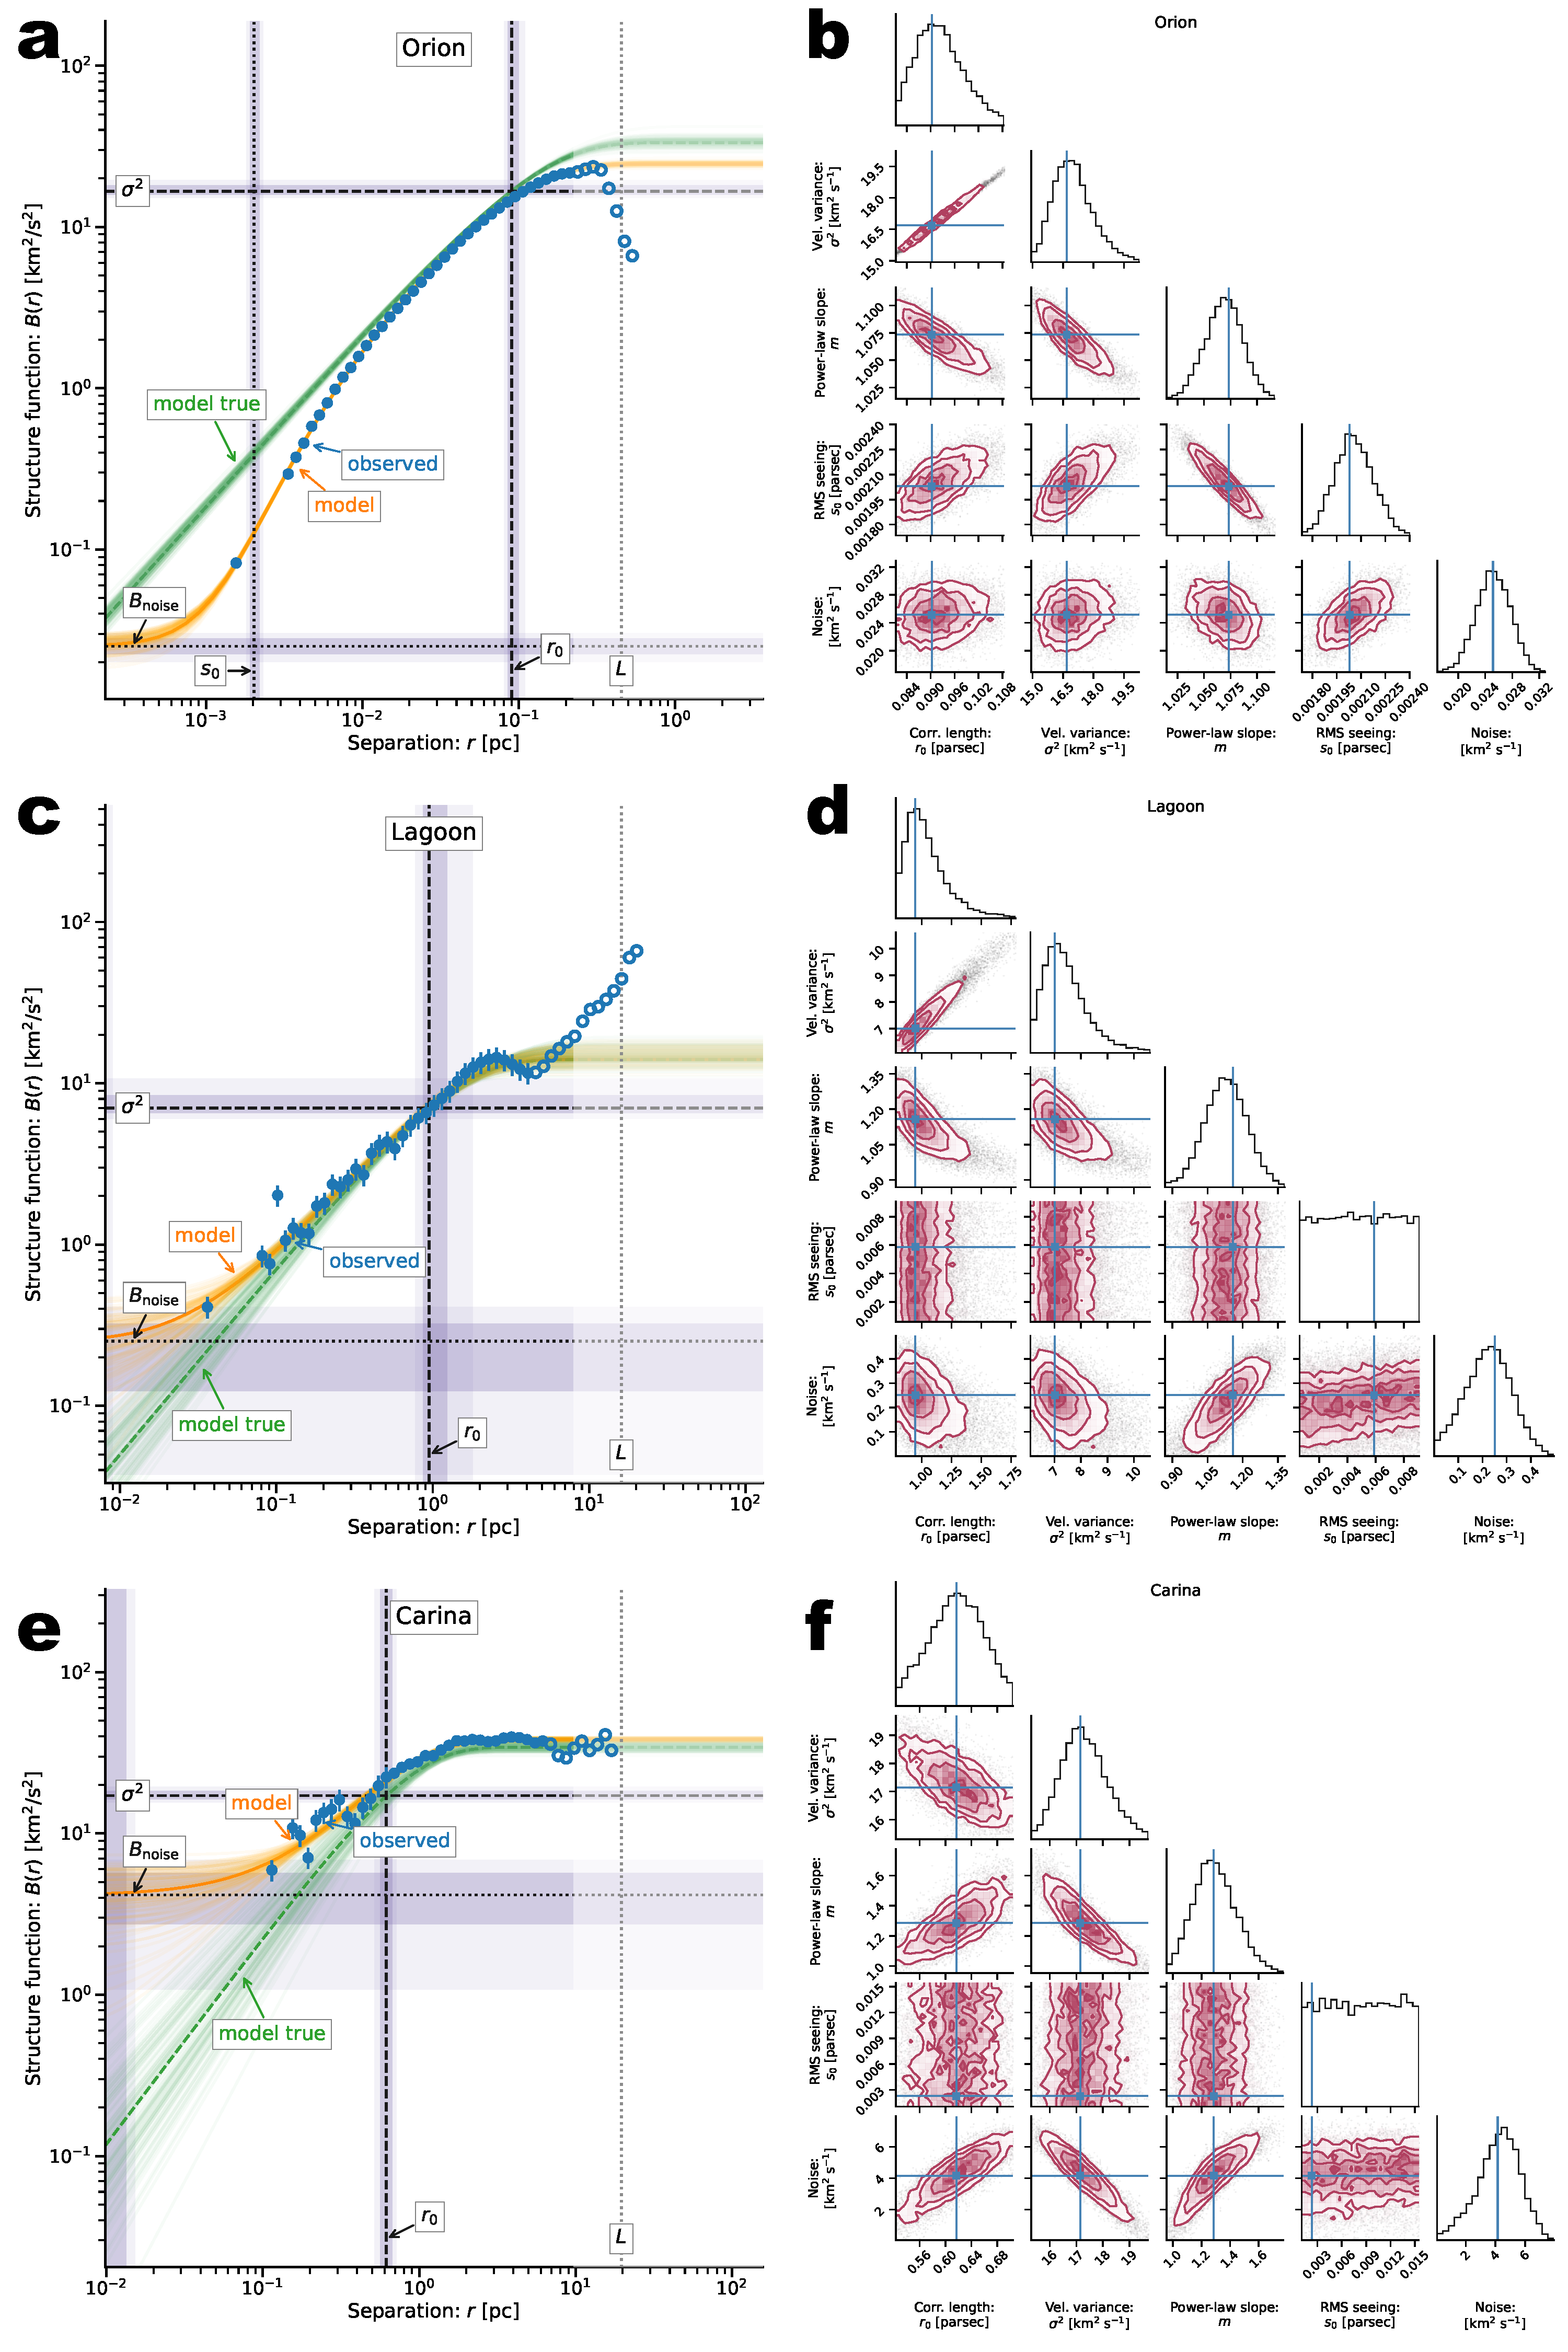
\includegraphics[width=0.8\linewidth]{Figures/strucfunc-fit-A}
  \caption{Second-order structure functions for the velocity centroid images of the \(H\alpha\) emission line}\label{fig:strucfunc-fit-A}
\end{figure*}

\begin{figure*}
  \centering
  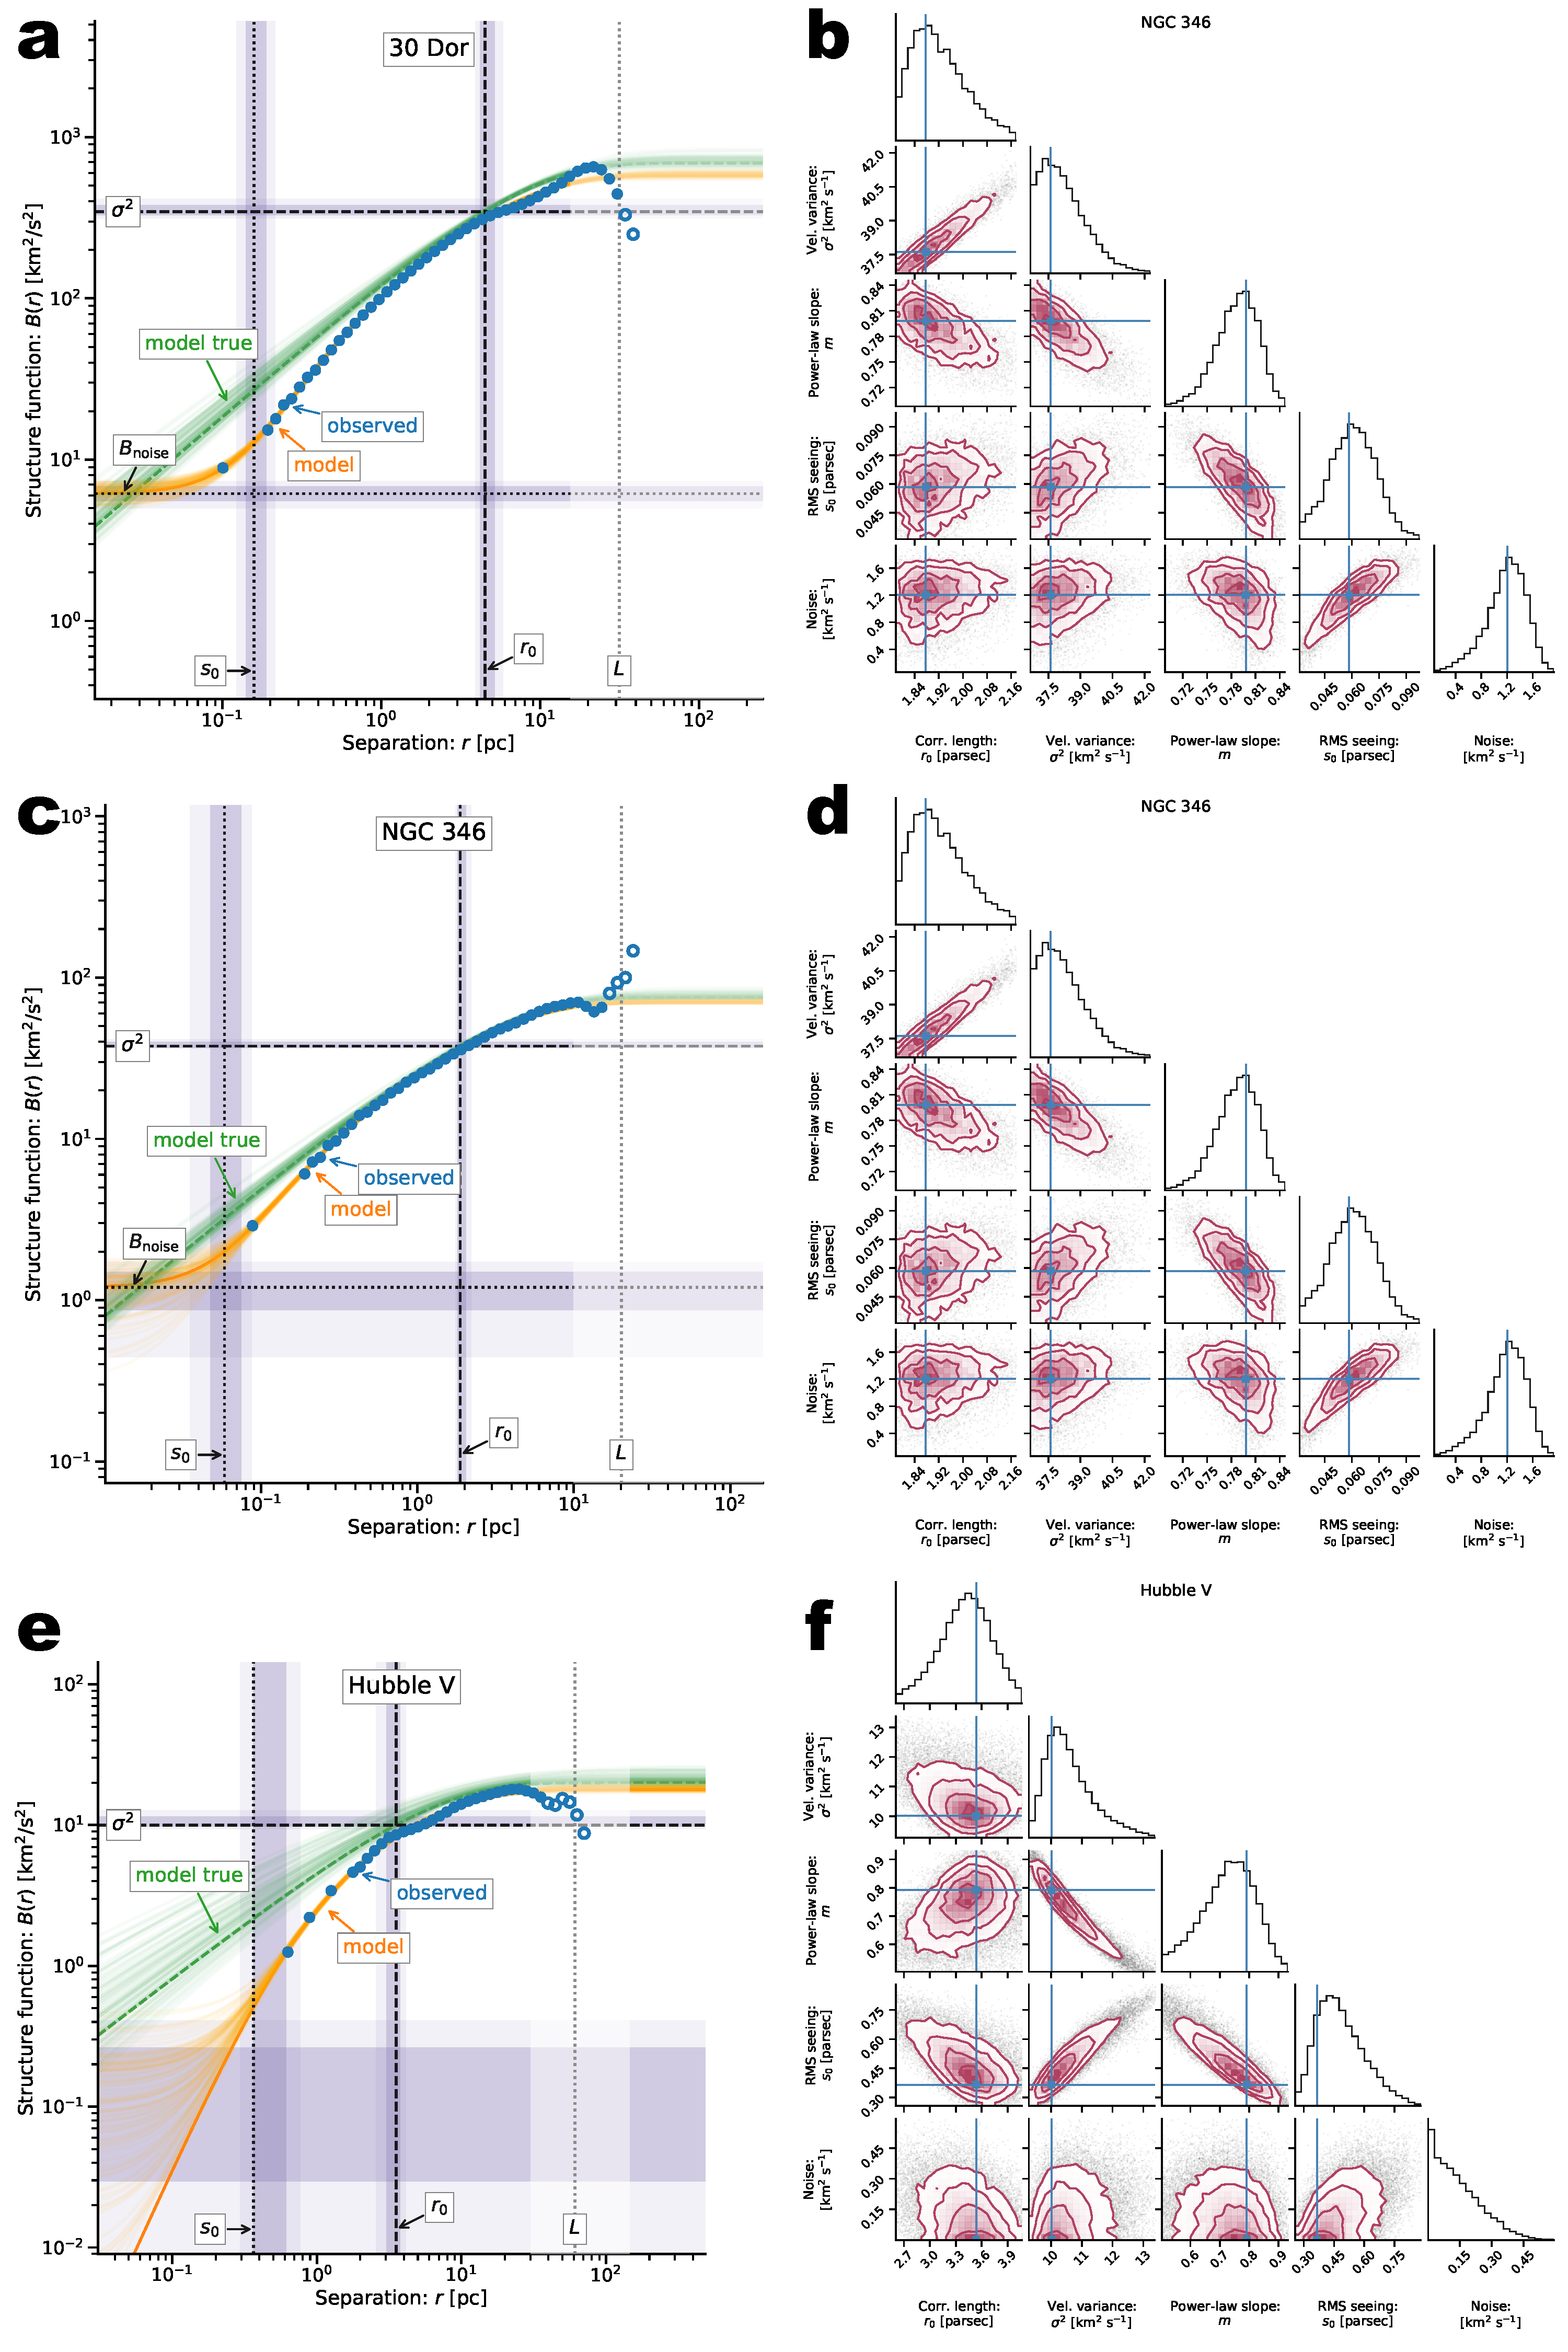
\includegraphics[width=0.8\linewidth]{Figures/strucfunc-fit-B}
  \label{fig:strucfunc-fit-B}
  \caption{Second-order structure functions for the velocity centroid images of the \(H\alpha\) emission line}
\end{figure*}

\begin{figure*}
  \centering
  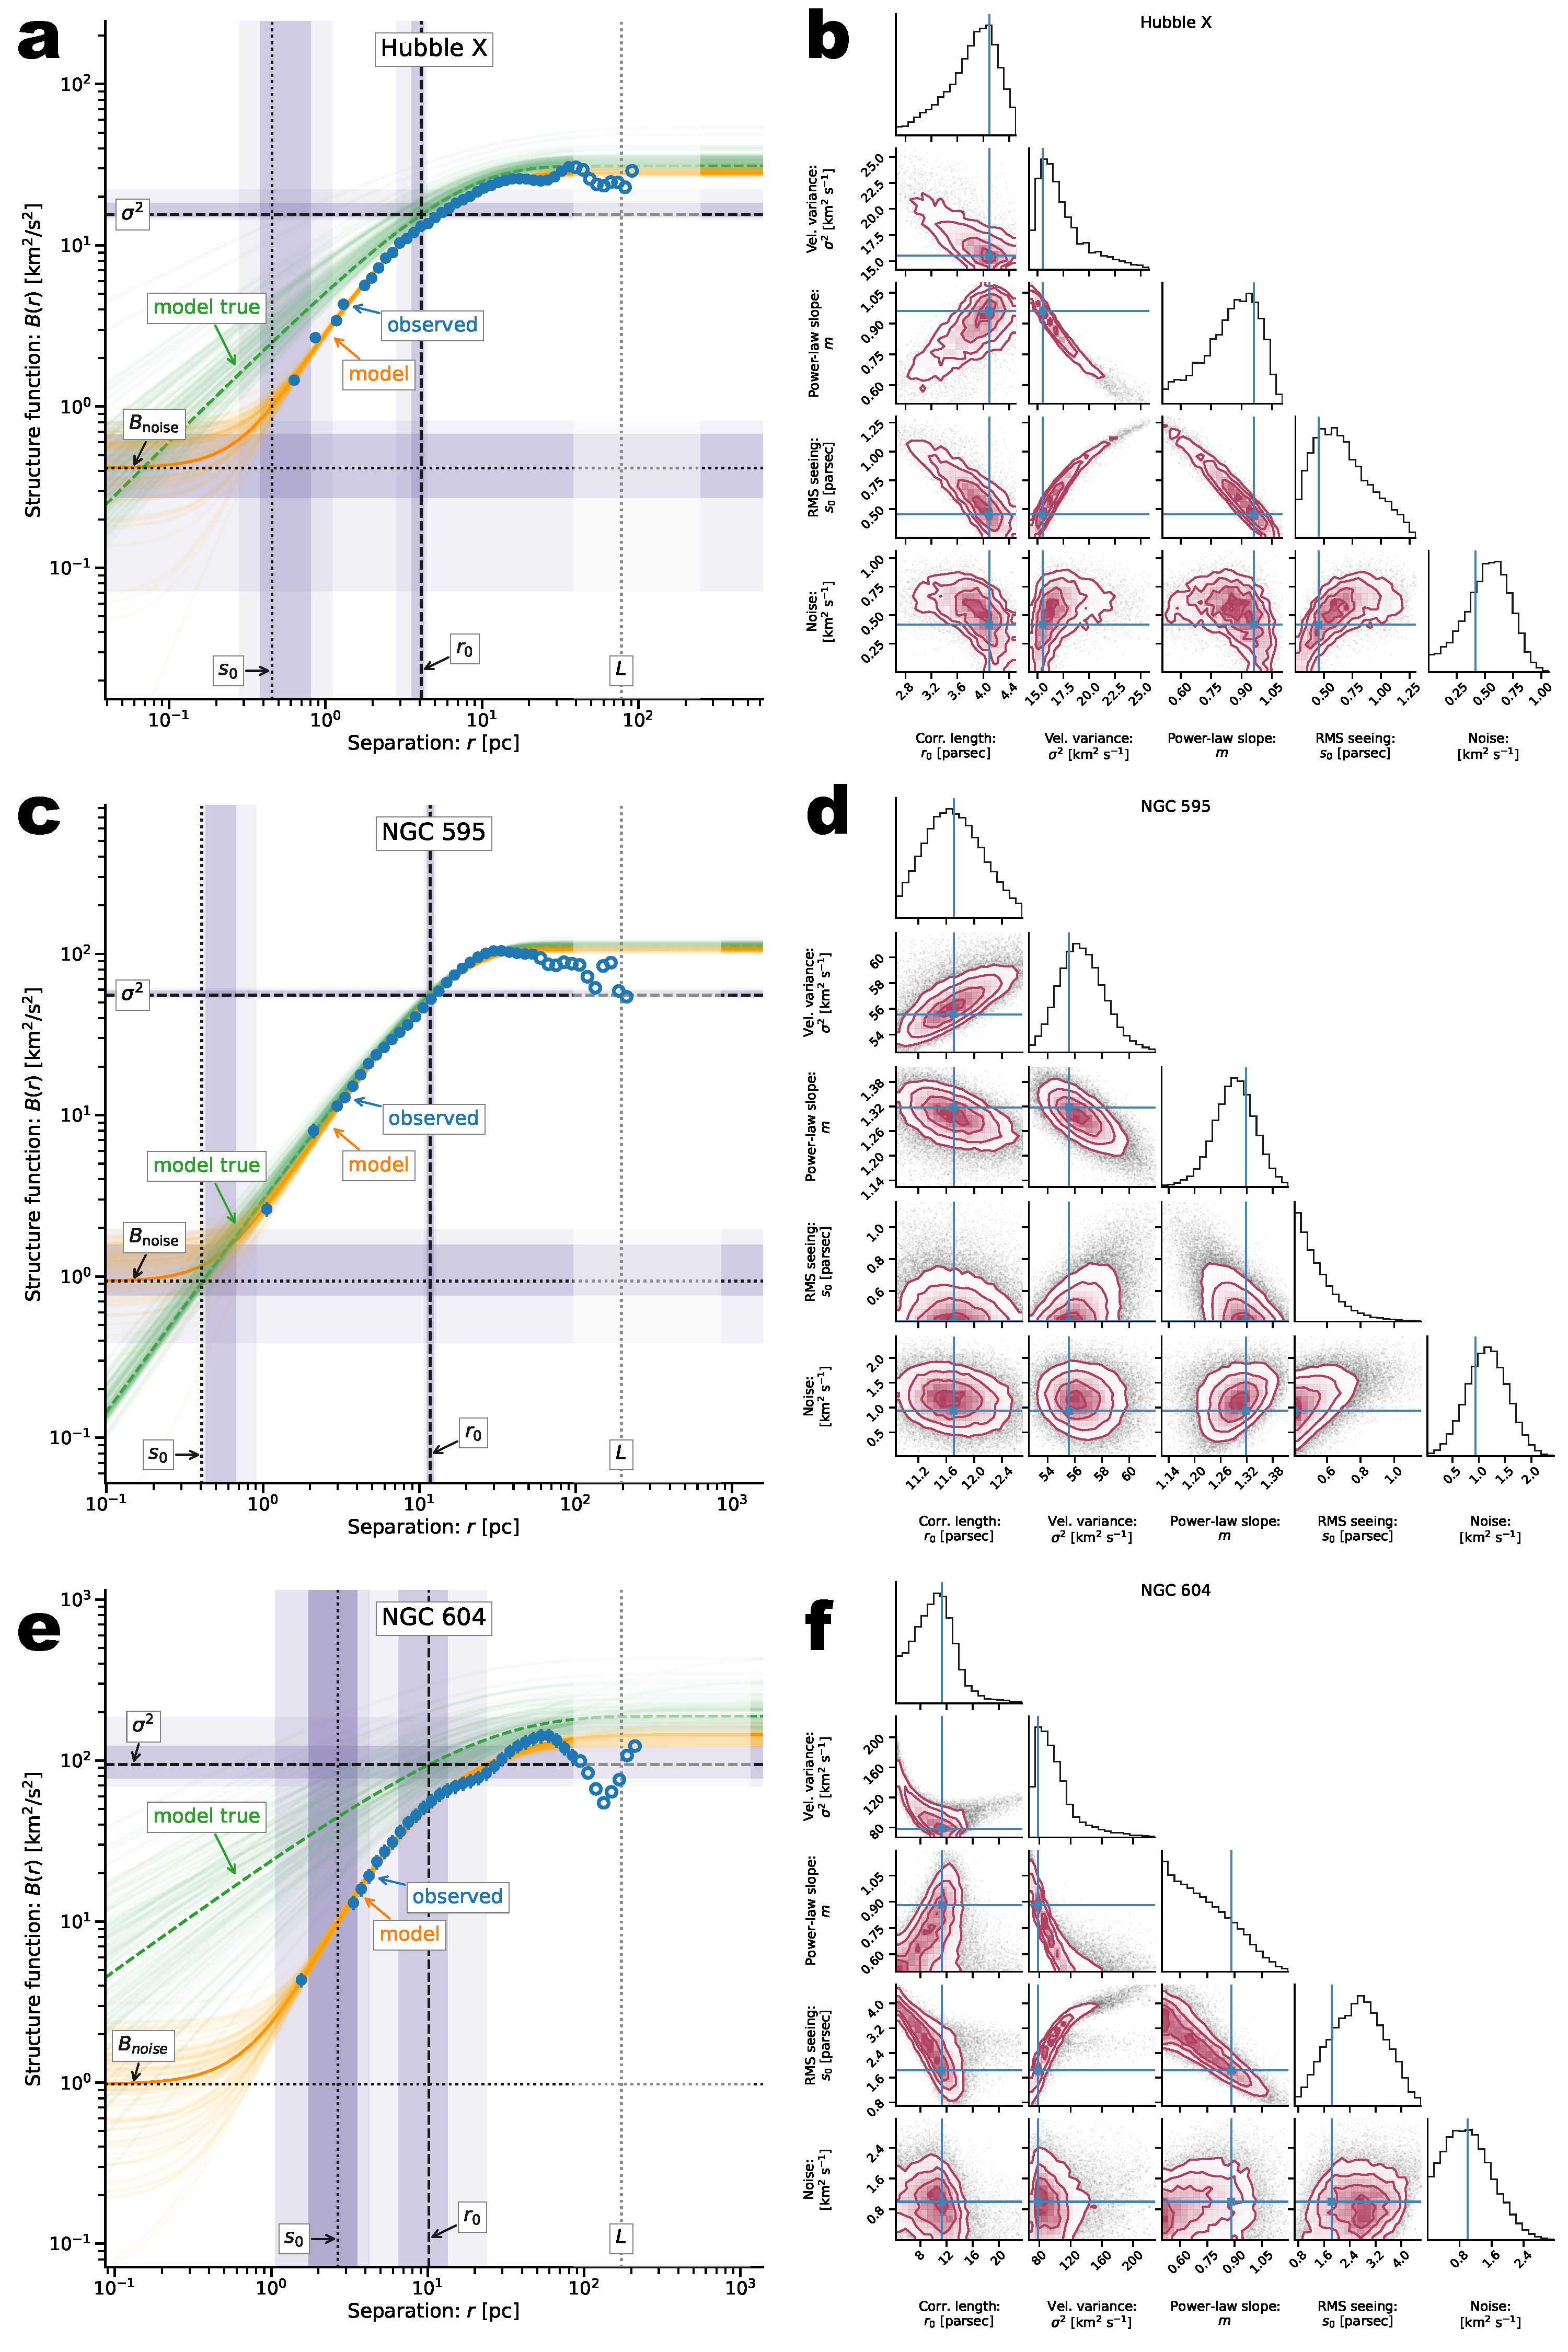
\includegraphics[width=0.8\linewidth]{Figures/strucfunc-fit-C}
  \caption{Second-order structure functions for the velocity centroid images of the \(H\alpha\) emission line}\label{fig:strucfunc-fit-C}
\end{figure*}

\begin{figure*}
  \centering
  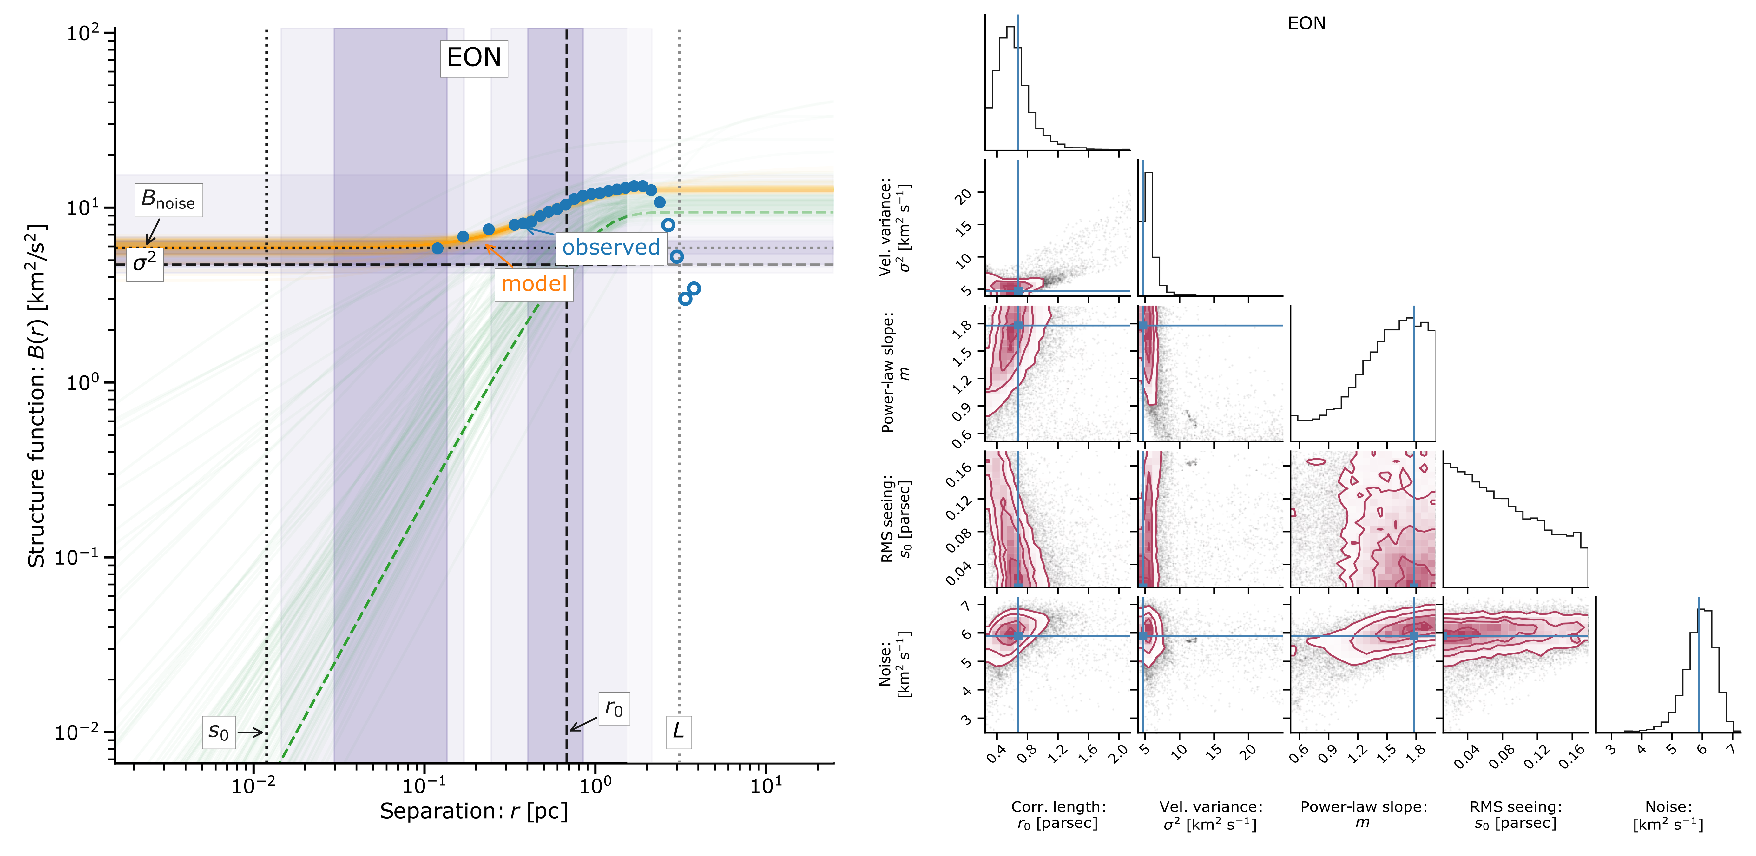
\includegraphics[width=0.8\linewidth]{Figures/strucfunc-fit-D}
  \caption{Second-order structure functions for the velocity centroid images of the \(H\alpha\) emission line}\label{fig:strucfunc-fit-D}
\end{figure*}

\begin{table*}
\begin{center}
\caption{Main results.}
\begin{tabular}{l CCCCCC}
\toprule
  Region &  \sigma^2\pos\quad [\si{km^2.s^{-2}}] 
         & B_{\text{noise}} \quad  [\si{km^2.s^{-2}}]  
         &  s0 \quad [\si{pc}] 
         &  r_0 \quad  [\si{pc}]
         &  L \quad [\si{pc}]
         & m  \\
\midrule
30 Dor &         300 \pm 9  &            6   \pm 1    &  0.16 \pm 0.02   &   4  \pm 0.2    &  32  &  0.84 \pm 0.04 \\
NGC 604 &         81 \pm 25 &            0.4 \pm 0.3  &   2.2 \pm 1.1    &   9  \pm 3.0    &  173 &  0.82 \pm 0.20 \\
NGC 595 &         56 \pm 2  &            1.2 \pm 0.4  &   0.5 \pm 0.1    &   12 \pm 1      &  196 &  1.3  \pm 0.05 \\
NGC 346 &         37 \pm 1  &            1.3 \pm 0.3  &  0.07 \pm 0.01   &   2  \pm 0.1    &  20  &  0.76 \pm 0.02 \\
Carina &          18 \pm 1  &              2 \pm 1    &  0.008 \pm 0.005 &  0.56\pm 0.04   &  20  &  1.14 \pm 0.10 \\
Hubble X &        16 \pm 2  &            0.5 \pm 0.2  &   0.6  \pm 0.3   &   4  \pm 0.4    &  78  &  0.88 \pm 0.14 \\
 Orion core &     13 \pm 1  &          0.025 \pm 0.002 & 0.002 \pm 0.0   &   0.07 \pm 0.01 &  0.5 &  1.07 \pm 0.02 \\
Hubble V &        10 \pm 1  &            0.1 \pm 0.1  &  0.5   \pm 0.1   &   3.4 \pm 0.3   &  61  &  0.74 \pm 0.1 \\
Lagoon &           7 \pm 1  &            0.2 \pm 0.1  &  0.005 \pm 0.003 &   1 \pm 0.2     &  16  &  1.13 \pm 0.1 \\
EON &              5 \pm 1  &              6 \pm 0.5  &  0.1   \pm 0.05  &   0.4 \pm 0.1   &  3   &  1.44 \pm 0.4 \\
\bottomrule
\end{tabular}\label{tab:Res}
\end{center}
\end{table*}

%%% Local Variables:
%%% mode: latex
%%% TeX-master: "strucfunc_paper"
%%% End:


%%%%%%%%%%%%%%%%%%%%%%%%%%%%%%%%%%%%%%%%%%%%%%%%%%%%%%%%%%%%%%%%%%%%%%%%%%%%%%%%%%%%%%

\section{Discussion}\label{sec:discussion}

\subsection{Turbulence}\label{sec:turbulence-theory}

\textit{Will 2021-12-10: Moving this section to later for now. Maybe
  this material could go in discussion.}

The idea to treat the ionized regions from a fluid mechanic view is intuitive if we consider the continuum hypothesis. 
We validate this hypothesis using the Knudsen number defined as \(Kn \equiv \lambda / l\), where \(\lambda\) is the mean free path of the medium and \(l\) a characteristic length of the phenomenon we are studying.
Taking into account a \(\lambda_{\text{HII}}\) of \SI{2.7e-7}{pc} \citep{1941ApJ....93..369S} and a \(l_{\text{HII}}\) of \SI{1}{pc} for ionized regions we obtained \(Kn \approx 10^{-7}\), while in general the continuum approach is valid for \(Kn \ll 1\).

A turbulent behavior in the flows is more common in fluid systems than a laminar one.
These turbulent flows tends to be unsteady, irregular and chaotic, and the turbulent motions are observed in many scales. 
The turbulent flows are associated with a high Reynolds numbers which is defined as \(Re = l v_{l} / \nu \), where \(v_{l}\) is a characteristic velocity in the fluid system and \(\nu\) is the kinematic viscosity of the medium.
Experiments have shown that a flow which is laminar become turbulent when increasing the velocity (i.e., increasing the \(Re\)) and a large range of velocity fluctuation appear at all scales.
A high \(Re\) reflects high ratio of the advection/difussion terms of the Navier-Stokes equations, being interpreted as that the inertial forces taking over the viscous ones. 
Hence it is possible to assume that if viscosity is not dominant in a flow, this flow would be turbulent.

As astronomical observation made it possible to measure a large number of points with a high accuracy, it was found that velocities show a non-thermal component reflecting characteristic of turbulent earthly flows.
The existence of turbulent flows in astrophysical objects, ranging in scales from 10\(^6\) to 10\(^{17}\) m \citep{2010ApJ...710..853C} is thought to be consequence of the high \(Re\), between 10\(^4\) and 10\(^9\) \citep{1949ApJ...110..329C,lagrois2011} that characterized these objects.

The classic turbulence theory assumes a three-dimensional isotropic, incompressible and subsonic flow that can be described using an energy spectrum formed by vortices or eddies of different sizes \citep{kolm1}.
The concept of the energy spectrum assumes that the energy is cascading down inside the flow from the largest to the smallest scales.
The different scales in the energy cascade are defined based on their \(Re\).
In one side of the spectrum there is the energy injection scale, \(L_I\), that is related to the largest vortices, called the integral scales, where \(Re \rightarrow \infty\).
On the other side of the spectrum there is the dissipation of energy at small scales, \(l_I\), where  \(Re \rightarrow 1\) and it is assumed that small vortices are responsible for the friction that dissipates the energy flux into thermal energy.
In between there is the inertial range, \(l_d  << l << L_I\), where in a stationary case the energy transfer is at a constant rate.

The rate of transfer of specific energy \(\epsilon\) (energy per unit mass) in the inertial range is independent of the \(l\) scale having the form \(\epsilon \sim v_l^2 / \tau_l\), where the kinetic energy is of the order of \( v_l^2\) and the life time of a velocity fluctuation is \(\tau_l\), which can be can be put in terms of \(\tau_l \sim l / v_l\). 
Hence we obtain \( v_l \sim (\epsilon l)^{1/3}\) where \(\epsilon\) is invariant in the cascade.

The energy cascade is described using the energy spectrum, $E(k) \propto k^{\beta}$ where \(k\) is the wave number for a determined scale \(l\) ($k \equiv l^{-1}$).
The total specific energy of a determined $l$ scale is of the order \(\langle v_{l}^{2} \rangle \) and is the energy integral above the associated \(k\), defined as:

\begin{equation}\label{eq:energy-spectrum}
 \langle v_{l}^{2} \rangle = \int_{k}^{\infty} E(k)dk
\end{equation}
%
If it is assumed that this energy is of the order of $(\epsilon l)^{\frac{2}{3}} \sim (\frac{\epsilon}{k})^{\frac{2}{3}}$ we can differentiate equation \ref{eq:energy-spectrum} and obtained the final form:

\begin{equation}\label{eq:kolmogorov-law}
E(k) \propto \epsilon^\frac{2}{3} k^{-\frac{5}{3}}
\end{equation}
%
where \(\beta = -5 / 3\) is the Kolmogorov law.
For supersonic turbulence the index is $\beta=-2$ \citep{burg}. 

Using a statistical law that relates the moments \(M_n\) of order \(n\) with the increments in the velocity field for a separation \(\boldsymbol{r}\) \citep{Leqism}, we have:

\begin{equation}\label{eq:velocity-moments}
M_n = \langle \vert \boldsymbol{v}(\boldsymbol{x} + \boldsymbol{r})- \boldsymbol{v}(\boldsymbol{x})\vert^n \rangle \propto (\epsilon r)^{n/3}
\end{equation}
the average is over all the positions \(\boldsymbol{x}\) and directions \(\boldsymbol{r}\). 
The Kolmogorov model predicts that the moment of order 2, the second-order structure function (equation \ref{eq:Br}), follows \(M_2 \propto r^{2/3}\).

These mathematical techniques were first applied to astronomical observations by \citet{von1951methode} and \citet{munch1958internal} allowing to determine a distinction between homogeneous turbulence and pure random velocity fluctuations in the Orion Nebula. 

\subsection{Interpretation of the turbulent parameters and origins of interstellar turbulence}\label{sec:interpretation-origin}
\textit{Note: Still working on this section}

The structure function used in this work does not reveal the precise characteristic of turbulence, but the statistical results that it provides allow us to determine a distinction between correlated or random velocity fluctuations in the photoionized gas, in which the presence of correlations in the velocity field is a inherent property of turbulence.
Although this work is not conclusive about the nature of photoionized gas turbulence and a precise description of the origin and implications of these turbulent motions is out of the scope of our investigation, we believe that the tools presented here (see section~\ref{sec:methods-apply}) guarantee a better approach to determine the structure function and a more concise way for a comparison of a sample of different regions.
The following sections addresses a vast series of turbulent problems that could be unravel by expanding the sample, among more kinematical research of each \hii{} regions.


\subsubsection{Correlation length \(r_0\)}

Ideally the correlation length \(r_0\) should represent the scale of dominant energy injection.
It is unclear what are the mechanisms driving the turbulence, thought a lot of options are candidates.
The main energy sources are, of the order of kpc, the differential rotations of the galaxy that produces shear at large scale, at scales of the order of hundreds of pc, supernova explosions inject a large amount of kinetic energy.
At scales of several tens of pc the expansion of \hii{} regions and stellar winds are also a source of energy and bipolar flows, shocks,jets and champagne flows inject energy at small scales, about one tenth of a pc.
The velocity fluctuations are consequence of the combination of the various mechanism already mentioned and wouldn't be correct to attribute these fluctuations solely to one mechanism.
The complexity of the extraction of pure turbulent motions from velocity profiles in nebulae is not just an observational problem, there is also the lack of precise information on how these mechanism contribute to the emission line broadening \citep{2011MNRAS.413..705L,arthur2016turbulence}. 

Many of the previous mechanisms, at least in some extent, affect all the \hii{} regions studied in this work.
It is possible to consider from our sample the smallest and largest regions for a comparison on the impact of the previous mechanism.
The Orion core is affected by the stellar wind from \(\theta^1\) Ori C \citep{2009AJ....137..367O} that will confine even the high ionization emission lines to a thick shell.
Orion also present a champagne flow where the photoionized gas streams away from the ionization front.
\citet{sabalisck1995supersonic} studied NGC 604 revealing that the kinematics of the region behave different considering different scales.
High emission knots on the region encompasses supersonic global velocity dispersion values of 14 $<$ \(\sigma_{\text{los}}\) $<$ \SI{20}{km.s^{-1}} with a characteristic radius of \(\sim\)\SI{7}{pc} and a Gaussian profile.
Values of velocity dispersion $>$\SI{20}{km.s^{-1}} are found in low emission cavities where the lines present strong asymmetries.
These cavities were identified as expanding shells \citep{yang1996} with diameters of \(\sim\)\SI{40}{pc} and a expansion velocity above \SI{50}{km.s^{-1}}

Although the Orion core and EON, and NGC 604 have different \(r_0\) is not clear if it truly reveal a concrete aspect of the energy input mechanism mentioned earlier.
Orion mainly energy input comes from one star, meanwhile NGC 604 has more than 200 OB stars including WR stars. 
The Orion core also presents Herbig-Haro objects, which aren't possible to resolve for more distant regions.
Though the correlation length is particular to each region, and it is correlated mainly with the size (see section~\ref{sec:scaling-relations}), it still needs further studies to reveal the true implication of this value with respect the energy input mechanisms.

\subsubsection{Structure function power-law index \(m\)}\label{sec:powe-index}

The index \(m\) shown in the last column of Table \ref{tab:Res} is used for comparison between observations and the theoretical value of 0.67 (equation \ref{eq:velocity-moments}).
All our indices are above this theoretical value and this is attributed to the fact that the analyzed regions do not comply with the assumptions established in the development of the turbulent theory.

From section~\ref{sec:regions-milky-way} we know that most of all assumption mentioned in section~\ref{sec:turbulence-theory} are not meet for our \hii{} region sample.
\hii{} regions emerged from a molecular cloud with highly filamentary and clumpy density structure .
There is a large increase in the temperature because of the photoionization and the density gradients with the pressure gradients accelerate the flow which occurs in multiple scale, consequence of the fractal nature of the molecular cloud \citep{arthur2016turbulence}.
The radiation pressure, stellar winds and region expansion, among other physical processes would create pressure-driven shock waves propagating faster than the speed of sound in the medium.
This would regard conditions in \hii{} regions as compressible and supersonic.
And as \hii{} regions are regarded as three-dimensional objects there is the possibility of a sheet-like distribution which could overcome this assumption.
%This would result in a inhomogeneous density structure where arcs, filaments and shells are characteristic of \hii{ } regions as we can see from Figure~\ref{fig:hii-regions}.

But despite the complex nature of \hii{} regions we observe a common pattern for the structure function and the value of the index we obtain falls in a certain limited range of values. 
The differences with respect the theoretical value are often used as a diagnostic tools to identify properties that are not consider in the assumptions of the turbulence theory.

For the comparison between the two-dimensional structure function and the three-dimensional structure function relationships between the power-law were proposed:

\begin{equation}\label{eq:projection-smearing-3d}
m_{2D}= m_{3D} + 1
\end{equation}
%
or when the astronomical object is almost two-dimensional (sheet-like):
%
\begin{equation}\label{eq:projection-smearing-2d}
m_{2D} \sim m_{3D}
\end{equation}

As a conclusion, if the extension of the HII region is compared with its depth (three-dimensional case) the value of the index is 1.6. 
While the case where the extension is much greater than its depth (two-dimensional case) the region will have a value of 0.6 \citep{von1951methode, munch1958internal,1987ApJ...317..686O}.

%We can compute the \(m_{3D}\) index from the two dimensional \(m\), if we assume that the \(m_{3D}\) index lies between the limits of projection smoothing and a sheet-like distribution. 
%Following the procedure by \cite{arthur2016turbulence} and assuming the relationship \(m_{2D} - 1 < m_{3D}\ < m_{2D}\) we have 0.54 \(< m_{3D} <\) 0.72.

\subsubsection{Relationship between plane-of-sky and line-of-sight velocity dispersion.}

%The broad in the velocity width of the emission line represents the range of velocities along the line-of-sight.%, among thermal movements. 
%We can consider as a main broadening mechanisms the kinematical disorder along the LOS related to %velocity gradients by the clumpiness on the molecular cloud and turbulent movements.
%On the plane-of-sky the consequences of those gradients and movements is measured in every pixel. 
%The spatial variations on the velocity field would depend on the targeted pixel, depending on the motions inside the cloud (the LOS component).
%This reasoning has lead to \citet{2011MNRAS.413..705L} to propose a direct relationship between \(\sigma_{\text{LOS}}\) and \(\sigma\pos\).

As a justification for the use of the structure function we can consider that any relation between the line width and line-of-sight depth can be interpreted in terms of a correlation between velocity spread and scale size.
This follows that if we have an optically thin spectral line where it will have a width which is related to the total radial velocity dispersion of all fluctuations sampled along the line-of-sight \citep{1984ApJ...277..556S}. 
In these sense the structure function is used as a tool to investigate the projection of a three-dimensional correlation function onto the plane of sky \citep{arthur2016turbulence}.

The standard deviation of the velocity centroid, \(\sigma\pos\), and the mean non-thermal linewidth, \(\sigma_{\text{LOS}}\), allow us to compare the relation between the kinematical disorder on the plane-of-the sky and along the line-of-sight  \citep{2011MNRAS.413..705L}.
It have been mentioned that the projection of the velocity fluctuations reduces the actual amplitude in the line-of-sight \citep{1984ApJ...277..556S,arthur2016turbulence}.

We can see from Table \ref{tab:Res} that the line-of-sight velocity dispersion is roughly twice the plane-of-sky velocity dispersion.

%In the case of homogeneous turbulent velocity we can consider the effect of \textit{project smearing} \citep{1984ApJ...277..556S}, where the projection from three to two dimensions over the line-of-sight depth \(H\), reduces the plane-of-sky amplitude for the condition \(r_{0} < H\).
%With a value of \(\sigma\pos / \sigma_{\text{los}}\) = 0.5 we obtain \(r_{0} / H \sim\) 0.02-0.1.

\subsection{Scaling relations between physical properties and turbulent parameters}\label{sec:scaling-relations}

In the section \ref{sec:results} we showed that each \hii{} region of our sample has a turbulent velocity field that can be characterized using the turbulence theory.
The turbulent parameters obtained are unique to each velocity field.
We proceed to develop scaling relations between them and also between the physical properties of each region.

%Intro for scaling relations
Relationship between the physical properties of \hii{} regions, like size and luminosity, and the velocity dispersion have been used as tools for concluding scaling relations for these objects.
These relations have also been studied in dwarf galaxies and high-redshift star formation regions.
\citet{melnick1977,terlevich1981} were the first to shown an empirical relationship between the line width and the integrated properties of the \hii{} regions as the diameter or the luminosity ($r \sim \sigma ^{\sim 2}$ ; $\text{L}_{\text{H}} \sim \sigma ^{\sim 4}$).
They conclude that GEHRs follow this relation because they behave as self-gravitatory systems like globular clusters or elliptical galaxies.
The work of \citet{1988A&A...201..199A} confirmed these relationships considering the discrepancies of previous investigations obtaining \(\text{L}_{\text{H}_{\alpha}} \propto \sigma^{3.9}\) and \(r \propto \sigma^{1.84}\).
%\citet{1981MNRAS.194..809L}

%Previous research on scaling relations
\citet{2012MNRAS.422.3339W} have found that clumps and \hii{} regions follow scaling relations over the range of z = 0-2 for \halpha\ size, velocity dispersion, luminosity and mass, finding \(\sigma \propto r^{0.42}\), \(\text{L}_{\text{H}_{\alpha}} \propto r^{2.72}\) and \(\text{L}_{\text{H}_{\alpha}} \propto \sigma^{4.18}\), respectively. 
This results imply that the same process are seen at high redshifts and the current epoch in star forming regions.
Recently, \citet{Moiseev:2015a} found that the relation in dwarf galaxies is \(\text{L}_{\text{H}_{\alpha}} \propto \sigma^{5}\).
\citet{2018MNRAS.474.1250F} presented the relationship between integrated H$_{\beta}$ line luminosity and the velocity dispersion for new data of 36 giant HII regions obtaining \(\text{L}_{\text{H}_{\beta}} \propto \sigma^{5.02 \pm 0.21}\).

%methods for our analysis
We follow through this analysis using the scaling relation as a research tool between the properties of the sample of HII regions and our results. 
We use the properties in Table \ref{tab:regions-properties} with the turbulent parameters in Table \ref{tab:Res} as the dependent variable to adjust a fit in the form \(Y = aX +b\). 
For this procedure we use a hierarchical Bayesian approach using the package \textit{linmix} \citep{2007ApJ...665.1489K}.
The results are shown in Table \ref{tab:RestStats} in ascending order for the p-value.
In the Figures \ref{fig:rvsR} and \ref{fig:sigvsl} we show the correlations with a significance level  $p < $0.05.
In all the figures the slope of the fit shown in solid black line is the mean of all red lines that reflect the posterior of the Bayessian analysis.

%Luminosity vs centroid velocity dispersion
The Figure \ref{fig:sigvsl} shows the log \(\sigma\pos\)-log \(\text{L}(\text{H}_{\alpha})\) plane.
Since this relation is the most common it can be use for comparison with the investigations mentioned at the beginning of this section.
Our results give us a relation of \(\log \sigma\pos = (0.28 \pm 0.1) \log \text{L}(\text{H}_{\alpha})-(10 \pm 4.0)\).
It is customary in the literature to present \(\text{L} (\text{H}_{\alpha})\) as the dependent variable.
In our case if we choose the upper uncertainty and take the inverse of slope we have \(\text{L}_{\text{H}_{\alpha}} \propto \sigma^{3.4}\). 
Using the same procedure in \textit{linmix} and changing the variables we obtained \(\log \text{L}(\text{H}_{\alpha}) = (3.1\pm 1.3) \log \sigma\pos -(36 \pm 1)\).
Both relations are close to the previously proposed \(\text{L}_{\text{H}} \propto \sigma^{4}\) relation.

%Size vs correlation length
The Figure \ref{fig:rvsR} shows the relation of the correlation length \(r_0\) and the size \(S\) of the region. 
The relationship we found is \(\log r_0 = (0.73 \pm 0.24) \log S - (1.17 \pm 0.5)\).
The values of the \(S\) are taken from \citet{1984ApJ...287..116K} and correspond to the outer
limits seen from visual inspection of the \ha{} photographs.
In this sense these values would represent an upper limit of the size of each region.
Since these objects do not posses a physical edges the size determination is not trivial.
Due to the above, we chose these set values since they come from an unique source and are foreign to our calculations and observations, which imply that there is no bias in the scaling law we obtain.  


\begin{table*}
\begin{center}
\caption{Linear regressions values in the form Y = aX + b between our turbulent parameters obtained using the chi-square statistic and properties of each region (Table \ref{tab:regions-properties}). The fifth column, $r$, is the Pearson correlation coefficient and the last column is the $p$-value. This results were obtained using the procedure in \citet{2007ApJ...665.1489K}.}
\begin{tabular}{RRRRRR}
  \toprule
  Y &                   X &                 a &                 b &       r &      p \\
  \midrule
  \log r_0 &         \log D_{\hii} &   0.95 \pm 0.33 &  -1.68 \pm 0.71 &   0.86 &  \mathbf{0.003} \\
  \log \sigma\pos &        \log L(\ha) &    0.25 \pm 0.11 &  -9.01 \pm 4.26 &   0.81 &  \mathbf{0.008} \\
  \sigma\los &  \sigma\pos &   1.03 \pm 0.45 &   7.40 \pm 2.88 &   0.78 &   \mathbf{0.010} \\[\smallskipamount]
  \log \sigma\pos &         \log D_{\hii} &   0.26 \pm 0.18 &   0.20 \pm 0.39 &   0.64 &   0.06 \\
  \log \sigma\pos &   \log r_{0} &    0.19 \pm 0.18 &   0.68 \pm 0.13 &   0.51 &  0.16 \\
  \log m &  \log d &  -0.02 \pm 0.04 &   0.04 \pm 0.08 &   -0.40 &   0.29 \\
  \log m &  \log  \sigma\pos &  -0.11 \pm 0.20 &   0.09 \pm 0.16 &  -0.37 &  0.33 \\
  \log m &  \log  r_{0} &   -0.02 \pm 0.07 &   0.02 \pm  0.05 &  -0.28 &  0.47 \\
  \bottomrule
\end{tabular}\label{tab:RestStats}
\end{center}
\end{table*}


%<10\(^{-5}\)

%%% Local Variables:
%%% mode: latex
%%% TeX-master: strucfunc_paper
%%% End:


\begin{figure}
\centering 
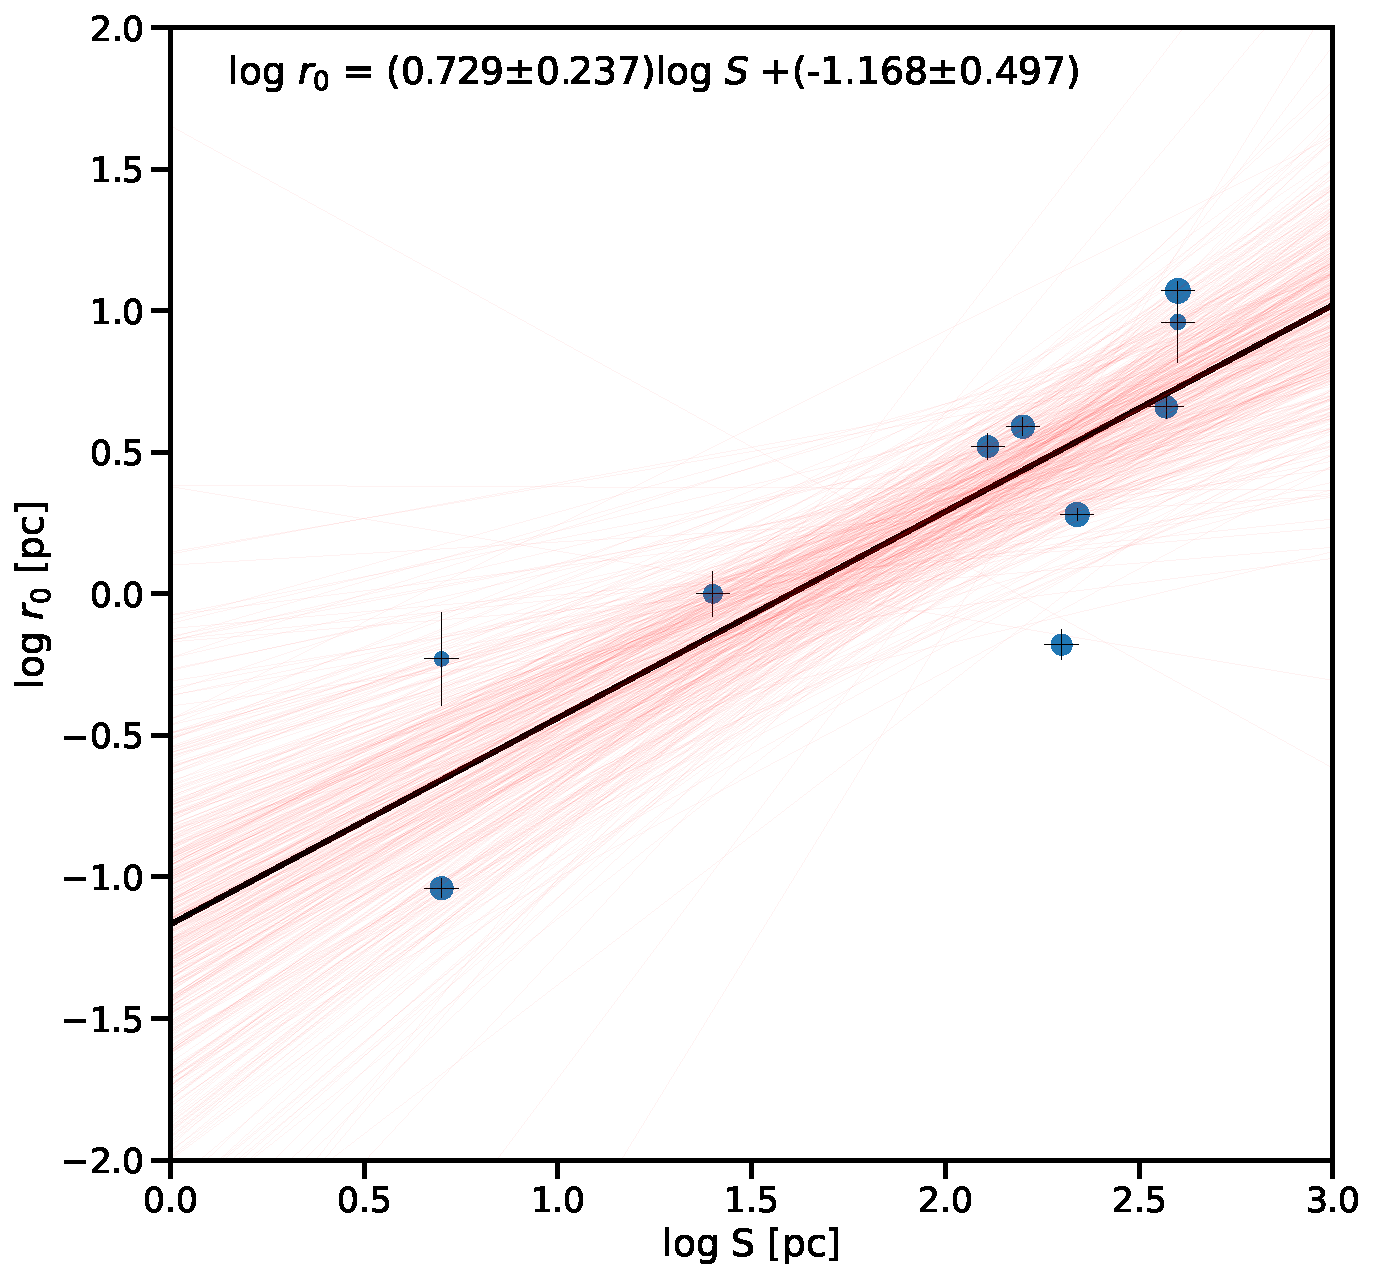
\includegraphics[width=3in]{Figures/rvsS}
\caption{The log \(r_0\) - log \(S\) plane derived form our results an data in the literature. A fit with slope of 0.67 $\pm$ 0.07 is shown in solid black line that is the mean of all red lines that reflect the posterior of the Bayessian analysis. }
\label{fig:rvsR}
\end{figure}

\begin{figure}
\centering 
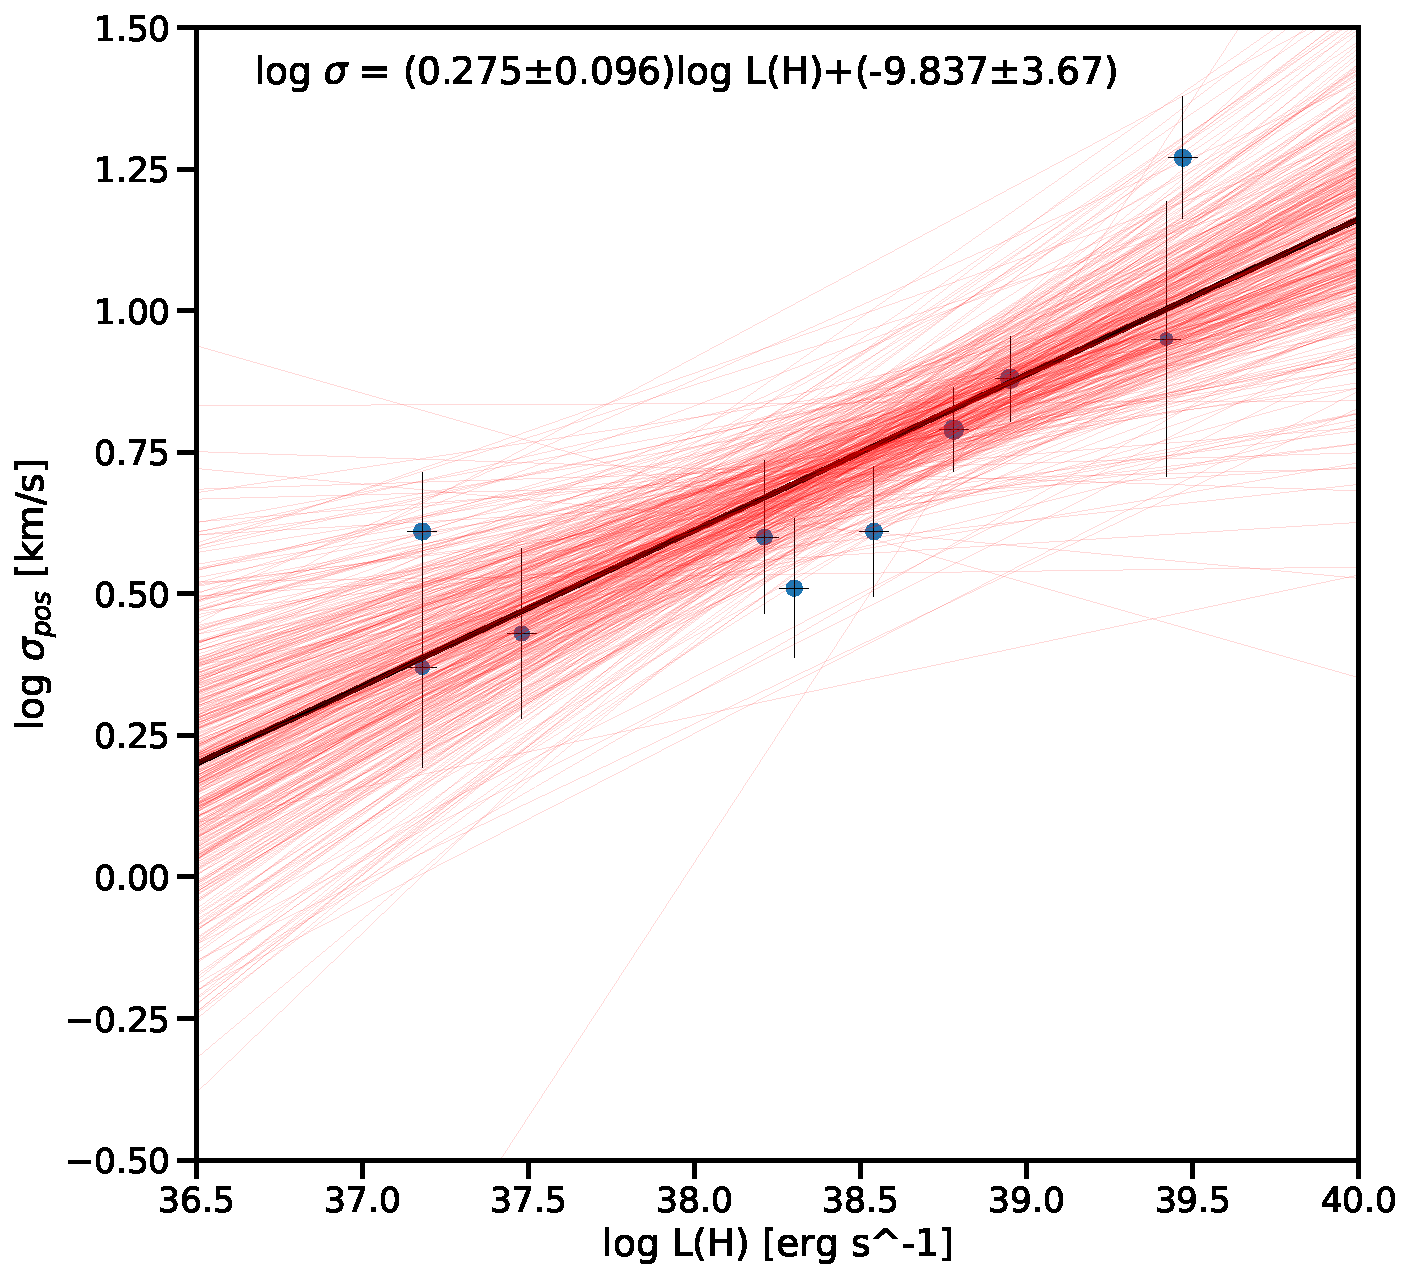
\includegraphics[width=3in]{Figures/svsL}
\caption{Same as Fig. \ref{fig:rvsR} but for the log $\sigma$-log $L(H_{\alpha})$ plane.}
\label{fig:sigvsl}
\end{figure}

%\begin{figure}
%\centering 
%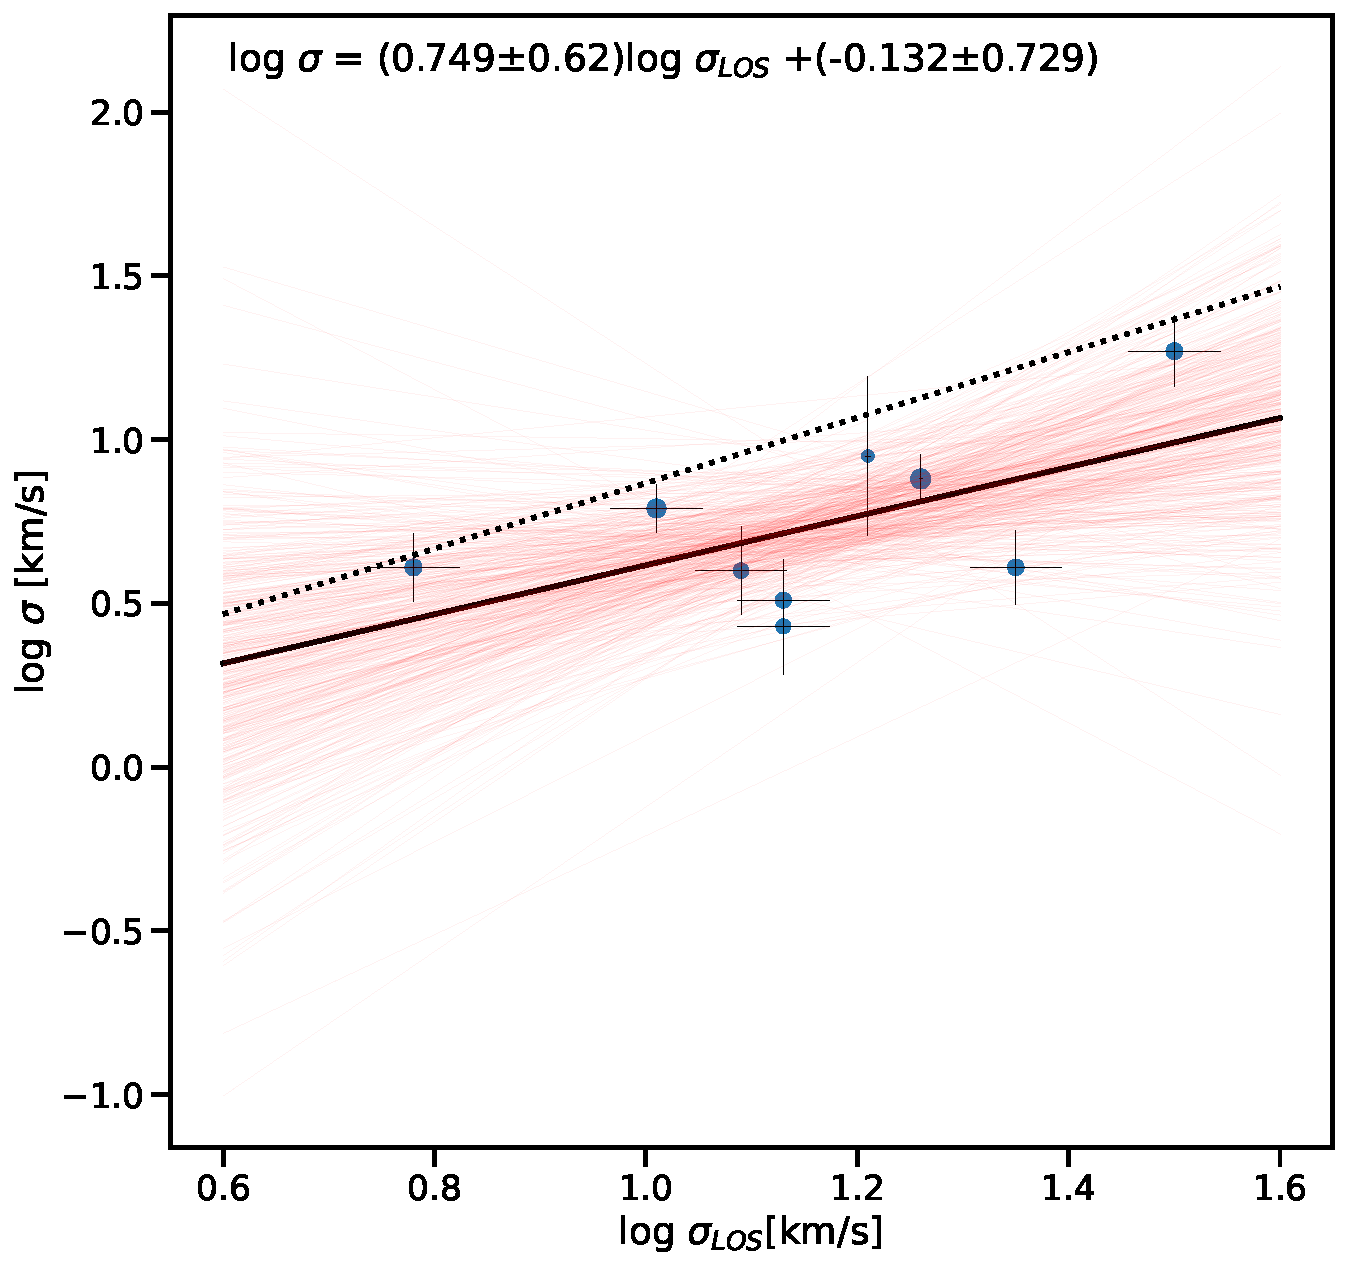
\includegraphics[width=3in]{Figures/svss.pdf}
%\caption{Same as Fig. \ref{fig:rvsR} but for the log $\sigma$-log $\sigma_{\text{LOS}}$ plane. The dotted line represents slope equal to unity.}
%\label{fig:svss}
%\end{figure}

\subsubsection{Kinematic relationship between ionized gas, molecular gas, and stars}
\label{sec:kinem-rela-betw}

Naively, the relatively small observed CO velocity dispersion
(\(\sigma(\chem{CO}) \ll \sigma(\ha)\) in all regions
for both \(\sigma\los\) and \(\sigma\pos\))
might be thought to rule out the molecular gas kinematics
as a \emph{cause} of the ionized gas kinematics.
However, this is not necessarily the case, so long as \emph{some} molecular gas
exists at the higher velocities typical of the ionized gas.

This is because a relatively small column of material
(\(N(\chem{H}) \sim \SI{e20}{cm^{-2}}\))
is sufficient to trap the ionization front,
in which case the \ha{} surface brightness is limited by the
incident ionizing flux
\citetext{the Ferland mechanism,
  see section~5.1 of \citealt{Baldwin:1991a}
  and section~B.2.1 of \citealt{Ferland:2012a}
}.
On the other hand, the bulk of the CO emission will come from much larger
column densities (\(N(\chem{H}) \sim \SI{e22}{cm^{-2}}\)),
where the molecules are effectively shielded from dissociation.
% If a given region can be considered as an ensemble of clouds of
% different masses, then ... would require lower mass clouds to move
% faster though, so needs dynamical relaxation

\textbf{Check  if this is actually feasible before developing further}

Very schematically, one could represent these processes as:
\begin{equation}
  \label{eq:1}
  \sigma^2(\ha) \sim \zeta \sigma^2(\chem{CO}) + \eta
\end{equation}
where \(\zeta\) is a multiplicative factor
due primarily to the saturation at the Ferland limit,
and \(\eta \sim \csound^2\) is an additive factor due to additional turbulence
generated by the transonic ionized photoevaporation flows.

\textbf{Estimate these two factors by fitting to the observations}

\subsection{Comparison with previous structure functions}

In Section \ref{sec:methods-apply} we mentioned the reduced chi-square method we are using for the determination of the correlation length and the index of the slope. Since this is the first time this method is applied to a sample of HII regions (at least for our knowledge), our results are bounded to be different from previous investigations, including the one that have the same observations as \citet{arthur2016turbulence} and \citet{2019arXiv191203543M}. 

A complete analysis on different emissions lines of the structure function on Orion was carried out by \citet{arthur2016turbulence} and reference therein. 
They observed a tendency that higher ionization lines presents higher values on the magnitude dispersion and the steepness of the structure function slope. 
This results just consider one component on the Gaussian fit. 
The power-law index obtained by \citet{arthur2016turbulence} are \(m \sim 1.2 \pm 0.1\) for \halpha\ and [OIII] emission lines and for [SII] they found \(m \sim 0.8 \pm 0.1\). 
The correlation length for all lines is \(\approx\) 0.05 pc. For the same \halpha\ observation we obtained a value of 1.06$\pm$0.01 and a correlation length of 0.092$\pm$0.007 pc. 

The first attempt at characterizing turbulence in a giant extragalactic HII region, GEHR, was done by \citet{1961MNRAS.122....1F} with the 30 Doradus complex in the LMC, finding no indication of turbulent motions between scale of 10 and 100 pc.
\citet{Melnick:2021x} also investigated the structure function in 30 Doradus finding on their results that the structure function is entirely flat on scales from 3 to 200 pc.
In the context of the high-resolution observations it is possible to see why their results do not reflect the turbulent structure of the nebula; their observations cover a region where the large-scale velocity fluctuations are uncorrelated.
There is a good agreement with the single-Gaussian fit results from \citet{2019arXiv191203543M} (Figure 15 Top on their work), while \citet{1961MNRAS.122....1F} results do not overlap with ours.
From this analysis this is the first time turbulence characterized in 30 Doradus using the structure function.

There is broad agreement in our structure function results and previous studies that consider NGC 604, mainly because where are using the same data \citep{Medina-Tanco:1997a, Melnick:2021x}.
From \citet{Medina-Tanco:1997a} and \citet{Melnick:2021x}, and using the same TAURUS-II data.
Despite this general agreement the interpretations in each study is different.
\citet{Medina-Tanco:1997a} conclude about a double regime acting on the kinetic energy spectrum.
According to this double cascading, turbulence is being forced at scales of \(\approx\)10 pc while and energy cascade has developed down to the smallest scales and other, as an inverse cascade, extends up to scale of \(\approx\)70 pc.
Interesting enough, \citet{Medina-Tanco:1997a} mentioned various characteristic scale lengths, the most notorious is the \(\approx\)10 pc, a value close to our correlation length of \(\approx\)9 pc, and they interpret it as possible source on energy associated with the expansion of shocks coming from wind bubbles.  
None of the previous studies present a power-law index for the structure function to compare our results.
\citet{Melnick:2021x} addresses some issues with TAURUS II data while comparing profiles between the previous instrument TAURUS I where there exist a difference between observations (see section 4.1 on their paper).
As we agree with them in the importance of observing NGC 604 at higher spatial resolution, we have prove that a consistent method in analyzing structure function is key to obtaining trustworthy results.

For our NGC 595 \halpha\ emission line results there is no correspondence in the structure function between our results and previous investigations.
Our observations cover the brightest part of the region and have smaller resolution.
\citet{lagrois2009multi} and \citet{lagrois2011} structure functions results does not cover scales $<$10 pc, where in our results the correlation is taking place.
\citet{lagrois2011} used the data from \citet{lagrois2009multi} to complement the structure function analysis with the auto correlation function and filters to the velocity field to get rid of non-turbulent movements.
Their sigma is 5.92$\pm$0.15 km/s with a correlation length is 43 pc and the power-law index they provide is 1.55$\pm$0.01.

%%%%%%%%%%%%%%%%%%%%%%%%%%%%%%%%%%%%%%%%%%%%%%%%%%%%%%%%%%%%%%%%%%%%%%%%%%%%%%%%%%%%%%%%%%%%%%%%%%%%%%%%%%%%%%%%%%%%%%

\section{Conclusions}\label{sec:conclusions}

The previous analysis was able to characterize the turbulence by determining a single inertial scale where the ionized gas behavior can be described by means of a power law.
To determine the inertial scale more precisely than in previous works, a new functional form was proposed for the second-order structure function that considers observational effects such as: seeing, noise and the size of the observational box.
These effects had not been considered in detail before and have important consequences in obtaining the inertial scale.

The new functional form of the structure function is used as an objective function in a non-linear regression to accurately determine the important parameters related to turbulence which are: the correlation length, the exponent of a power law that fits the results and the real variance of the region.

This proposed analysis can be expanded to other HII regions with the possibility of comparing the results between them since the method guarantees homogeneity and the ability to develop a future catalog of these regions in a coherent way.
It could even be used to investigate the velocity fields of other phases of the interstellar medium.
The study of turbulence between ionized regions and the molecular clouds that give them birth can be carried out in a concise way, having the correct methods with the intention of advancing the understanding of the kinematic relationships between them.

\begin{enumerate}
\item For 30 Doradus with an observational box size of 32 pc an index of 0.84$\pm$0.03 is obtained with an inertial scale between 0.1 and 5 pc, and with a variance of 350$\pm$21 km$^2$/s$^2$. 
    
\item For NGC 604 with an observational box size of 173 pc an index of 0.82$\pm$0.20 is obtained with an inertial scale between 2 and 9 pc, and with a variance of 81$\pm$25 km$^2$/s$^2$.
    
\item For NGC 595 with an observational box size of 196 pc an index of 1.3$\pm$0.04 is obtained with an inertial scale between 0.5 and 12 pc, and with a variance of 56$\pm$1.6 km$^2$/s$^2$.

\item For NGC 346 with an observational box size of 20 pc an index of 0.78$\pm$0.02 is obtained with an inertial scale between 0.06 and 2 pc, and with a variance of 38$\pm$1.0 km$^2$/s$^2$.

\item For Orion with an observational box size of 0.45 pc an index of 1.06$\pm$0.02 is obtained with an inertial scale between 0.002 and 0.09 pc, and with a variance of 17$\pm$1.0 km$^2$/s$^2$.

\item For Carina with an observational box size of 20 pc an index of 1.36$\pm$0.30 is obtained with an inertial scale between 0.008 and 0.6 pc, and with a variance of 17$\pm$1.0 km$^2$/s$^2$.

\item For Hubble X with an observational box size of 78 pc an index of 0.94$\pm$0.12 is obtained with an inertial scale between 0.5 and 4 pc, and with a variance of 15.5$\pm$1.5 km$^2$/s$^2$.

\item For Hubble V with an observational box size of 61 pc an index of 0.72$\pm$0.09 is obtained with an inertial scale between 0.5 and 3 pc, and with a variance of 10.6$\pm$0.8 km$^2$/s$^2$.

\item For Lagoon with an observational box size of 16 pc an index of 1.12$\pm$0.09 is obtained with an inertial scale between 0.005 and 1 pc, and with a variance of 7.2$\pm$0.8 km$^2$/s$^2$.


    
\end{enumerate}

%%%%%%%%%%%%%%%%%%%%%%%%%%%%%%%%%%%%%%%%%%%%%%%%%%%%%%%%%%%%%%%%%%%%%%%%%%%%%%%%%%%%%%%%%%%%%%%%%%%%%%

\section*{Acknowledgements}

Based on observations made with KPNO telescopes
\textit{complete KPNO acknowledgment}.
Based on observations made with ESO Telescopes at the La Silla Paranal Observatory under programme IDs 076.C-0888 and 098.D-0211.
Based on observations made as part of the Gaia-ESO Spectroscopic Survey
\textit{complete Gaia-ESO acknowledgment}.
Based on observations made with the WHT
\textit{complete WHT acknowledgment}.
We are grateful to Norberto Castro Rodríguez for providing maps of emission line velocity moments for 30 Doradus derived from MUSE-VLT observations.
JGV acknowledges and thanks CONACyT-Mexico for the PhD research scholarship.

%%%%%%%%%%%%%%%%%%%%%%%%%%%%%%%%%%%%%%%%%%%%%%%%%%
%%%%%%%%%%%%%%%%%%%% REFERENCES %%%%%%%%%%%%%%%%%%

\bibliographystyle{mnras}
\bibliography{bibphd}

%\clearpage

%%%%%%%%%%%%%%%%%%%%%%%%%%%%%%%%%%%%%%%%%%%%%%%%%%
%%%%%%%%%%%%%%%%% APPENDICES %%%%%%%%%%%%%%%%%%%%%
%%%%%%%%%%%%%%%%%%%%%%%%%%%%%%%%%%%%%%%%%%%%%%%%%%

\appendix

\section{Degradation of the structure function due to observational limitations}
\label{sec:degr-struct-funct}
Studied in context of \(\Delta\)-variance by \citet{Bensch:2001l}.

For a correct analysis on the structure function it is necessary to consider the consequences that the observational box size and the seeing have on the results.
To quantify the impact of these considerations on the final structure function, we perform a series of experiments using artificial turbulent velocity maps.
In particular, our interest is to quantify how this observational limitations affect the determination of parameters such as the correlation length, \(r_0\), and the velocity field variance, \(\sigma^2 \). 

The artificial velocity maps are created using a modified version of the \textit{make$\_$extend} command from the \textit{turbustat} package \citep{Koch2019AJ....158....1K}.
We create a turbulent velocity field that follows a given power law with and a proposed correlation length, and a variance value indicated as true \(\sigma^2\).
Using this true \(\sigma^2\) we obtained the true \(r_0\), and these values are used as a reference in the following experiments to quantify the variations.
The objective is to create a sample of multiple divided maps with different seeing width to compute the structure function in each and characterize the variations. 

\subsection{Finite box effects}
\label{sec:finite-box-effects}

The Figure \ref{fig:finite-box}a shows some of the simulated velocity fields we use to study the variations in the structure function with respect to the size of the observational box.
Initially we have an original field of \(512 \times 512 \) pixels that are divided \(n\) times and produce \(N = 4^n\) fields, where each one has a linear size \(L \times L \) with \(L = 2^{9 -n}\).
The structure function is calculated for each division and later we average all the divisions of the corresponding map. 

The Figure \ref{fig:finite-box}b shows in solid lines the normalized averaged structure functions for the maps in Figure \ref{fig:finite-box}a.
The number \(N\) of divisions and the length \(L\) are indicated in each structure function.
The shaded areas show the deviation that each average structure function has due to the different divisions. 
\textit{(Note: I modified the Figure adding \(\sigma^2\) and \(r_0\) for each SF since I think it is easier and more directly to grasp the effect of reducing the box size. The figure is more 'noisy' but if it seems like it contribute to nothing we can change it back.)}

The blue horizontal and vertical dashed lines show the true \(r_{0}\) and the value of \(B(r) / \sigma^2 = 1 \), respectively.
The colored dotted lines indicate the averages, taking into account all the divisions of each map, of the apparent \(r_ {0}\) and the apparent \(\sigma^2 \).
From this analysis it is clear that \(r_0\) and \(\sigma^ 2 \) decrease with respect to the true values as the size \(L\) of the observational box decreases. 
This analysis is performed on different maps (no images are shown) given a different power law in the velocity spectrum and different correlation lengths, giving the same results. 

Figure \ref{fig:finite-box-effect} shows the ratio of the correlation length of each averaged map with respect to the true correlation length, \(\text{apparent } r_ 0 /\text{true } r_0 \), as well as the ratio between the averaged variance of each divided map and the true variance, \(\text{apparent } \sigma^2  / \text{true } \sigma^2\).
We observe that for the values where \(L\), is 20 $> r_0 $ the change in the ratios is null.
It is for the values where \( L < 10 r_0 \) a considerable decrease in both ratios is observed.
This behavior is fulfilled for all simulated maps with different power law in the velocity spectrum and different correlation functions, indicated with different colored circles in Figure \ref{fig:finite-box-effect}. 
These variations of the ratios are used to characterize the effect that the decrease of the observational box size has in \(r_0\) and \(\sigma^2\).

The fitted dashed line in Figure \ref{fig:finite-box-effect} is given by the equation: 

\begin{equation}\label{eq:ajustebox}
\beta(r_0) = 1 - exp \left[ \frac{L}{3.6r_0} \right] 
\end{equation}
%
and it is used in the functional form that fits the observational structure function when adjusting the results to obtain the reported parameters \(r_0\) and \(\sigma^2 \). 

\begin{figure}
  \begin{tabular}{@{} l @{}}
    (a)\\
    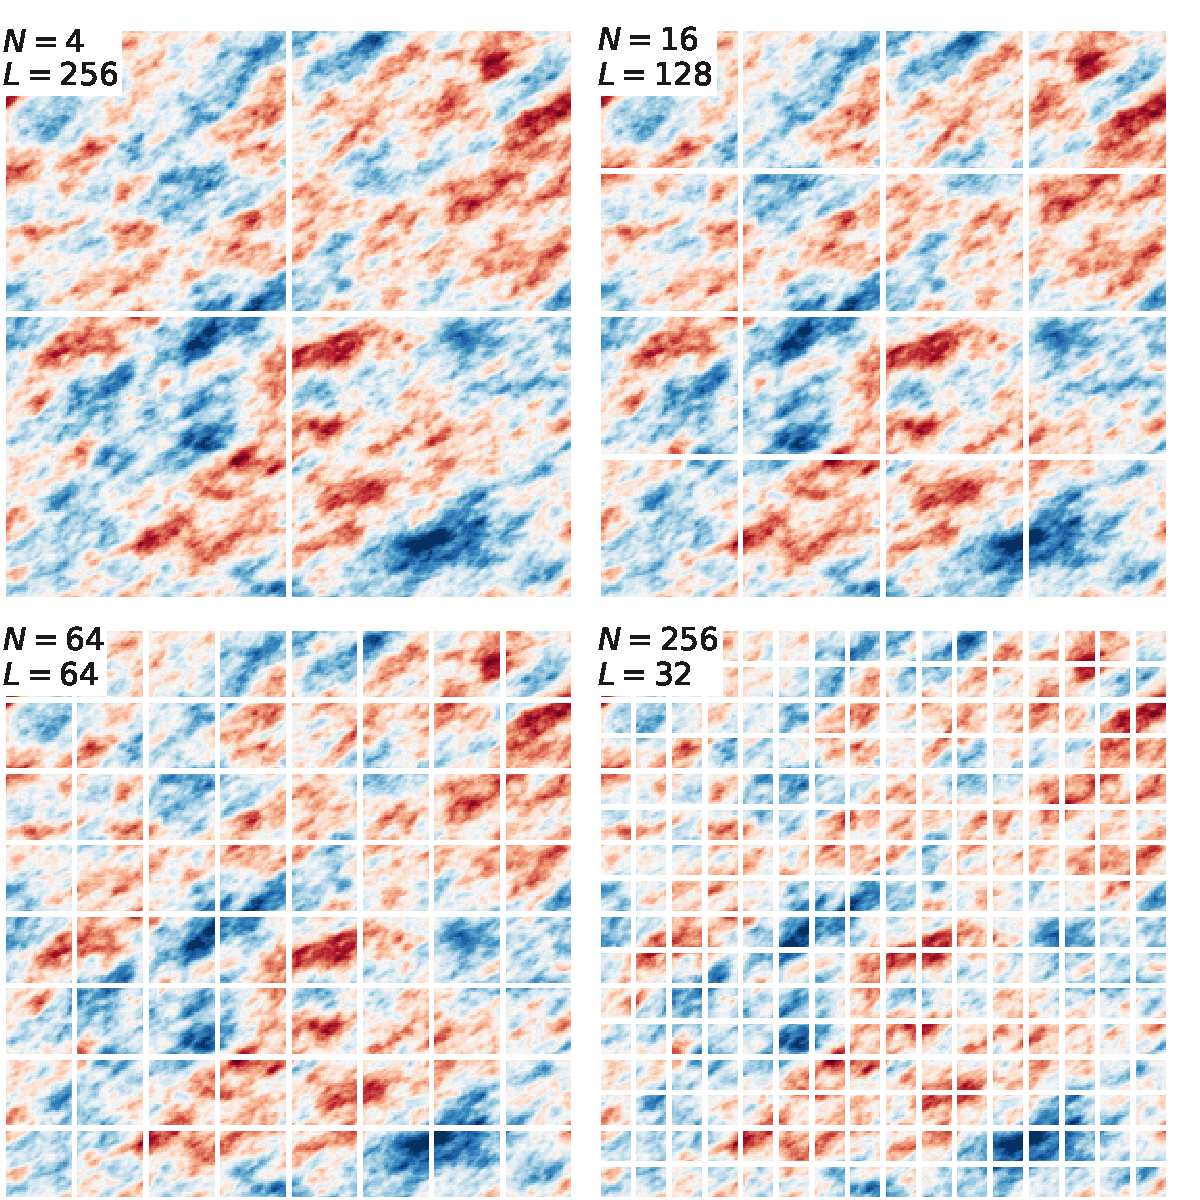
\includegraphics[width=\linewidth]{Figures/fake-finite-box-images}
    \\[\bigskipamount]
    (b)\\
    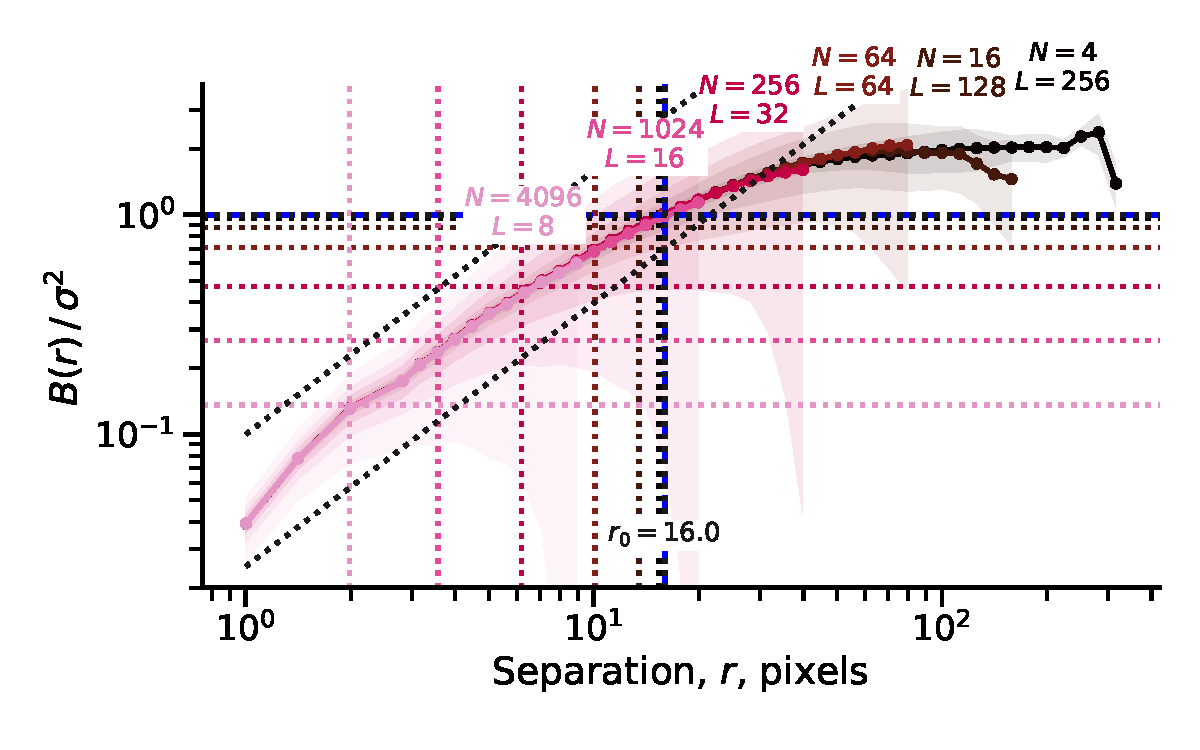
\includegraphics[width=\linewidth]{Figures/fake-finite-box-strucfunc2}
  \end{tabular}
  \caption{Effects of finite box size on the structure function.
    (a)~Construction of simulated turbulent velocity fields of different sizes
    by repeated division of an initial field of size \(512 \times 512\) pixels.
    The \(j\)th level of division yields \(N = 4^j\) fields,
    each of linear size \(L \times L\) where \(L = 2^{9 - j}\). 
    (b)~Resultant structure functions.
  }
  \label{fig:finite-box}
\end{figure}

\begin{figure}
  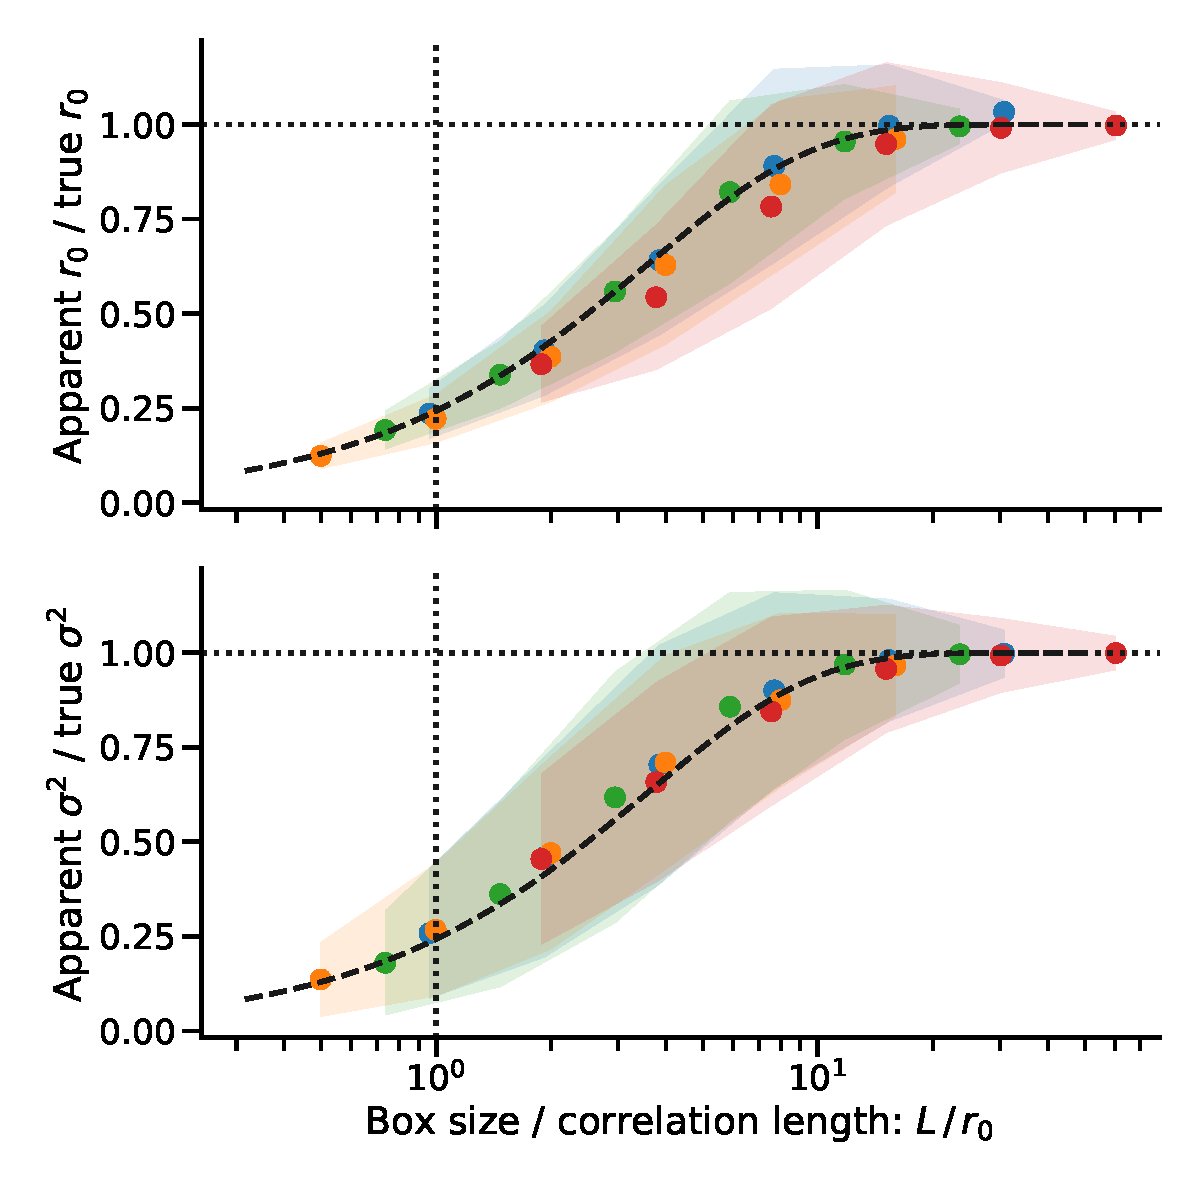
\includegraphics[width=\linewidth]{Figures/fake-finite-box-effect}
  \caption{
    Reduction of apparent velocity variance and correlation length
    due to finite box size.
  }
  \label{fig:finite-box-effect}
\end{figure}



\subsection{Effects of seeing}
\label{sec:effects-seeing-struc}

Ground-based astronomical observations are affected by the seeing produced by the atmosphere.
When calculating the structure function of these observations, this seeing affects the results at small-scale separations due to the smoothing of velocity fluctuations between adjacent pixels.
To study the consequences of the seeing we calculate the structure function of velocity maps where an artificial Gaussian seeing with different line widths has been introduced.
The artificial velocity maps are created in the same way as to study the effect of the observational box.
Seeing in velocity maps is added via the \textit{astropy} package using the \textit{Gaussian2DKernel} command. 

The rows in Figure \ref{fig:seeing-reduction}a show a synthetic velocity field of 512 \(\times\) 512 divided into four maps of 256 \(\times \) 256.
The color scale is the same for all maps and it considers \(- 3\) to \(+ 3\) times the standard deviation.
A Gaussian seeing, \(s_0 \) is applied to each division, with an RMS width ranging from 1 to 32 pixels, shown in the columns of Figure \ref{fig:seeing-reduction}. 
The structure function is computed in these maps and the averaged considering the same seeing. 

The solid lines in Figure \ref{fig:seeing-reduction}b  show the ratio of the structure function of the averages of the maps with their respective seeing and the map without it: \(B (r, s_0 ) / B (r, s_0 = 0) \).
The circle symbols indicate the value of 2\(s_0\) while the plus symbols indicate the apparent correlation length of smoothed map.
The vertical dotted line indicates the true \(r_ {0} \). 

The dashed lines in Figure \ref{fig:seeing-reduction}b are  empirically fits for each ratio.
To obtain this fit, we start from a convolution of an emission line and Gaussian seeing.
The emission line has the form \(\text {I}(x, v) = \text{I}_0 \phi [v; \overline {v} (x), \sigma_0]\) and has uniform width and brightness where the only change with respect to position is the velocity centroid.
The proposed seeing is \(\text{K}(x, s_0)\) of the form \(1 / \sqrt{2 \pi s_0} \exp^ {-x^ 2 / 2s_0 ^ 2} \).
The convolution \(\text{I}(x, v) \otimes \text{K}(x, s_0) \) is performed to obtain the smoothed map, \(\text {\~I} (x, v) \). 

Then we calculate the average velocity difference of the original map, \(\Delta v \), and the smoothed map, \(\tilde{\Delta v}\), in the points \( x = \{0, \delta \} \).
This expansion gives a term that modifies the final form of the structure function, \(~B (r)\), where the structure function without the seeing, \(B(r) \), is corrected by the term \(S_0(r; s_0)\) which has the form: 

\begin{equation}\label{eq:seeingcon}
S (r;s_0) = \tanh^2 \left[ \left( \dfrac{r}{2s_0} \right)^2 \right]
\end{equation}

Subsequently, the equation \ref{eq:seeingcon} is empirically modified and we obtain: 

\begin{equation}\label{eq:seeingemp}
S(r; s_0, r_0) =  \frac{e^\frac{-s_0}{r_0}}{2} \left(1 + \tanh{a \text{ln} \frac{r}{2s_0}} \right)
\end{equation}
%
and the final form of the equation \ref{eq:seeingemp} after a mathematical simplification gives: 

\begin{equation}\label{eq:seeingemp2}
S(r; s_0, r_0) = \frac{e^\frac{-s_0}{r_0}}{1+(\frac{2s_0}{r})^{2a}}
\end{equation}
%
which describes the fit (dashed lines) in Figure \ref{fig:seeing-reduction}b. 

The equation \ref{eq:seeingemp2} is used to correct the observational structure function, \(B(r)\). 

\begin{figure}
  \begin{tabular}{@{} l @{}}
    (a)\\
    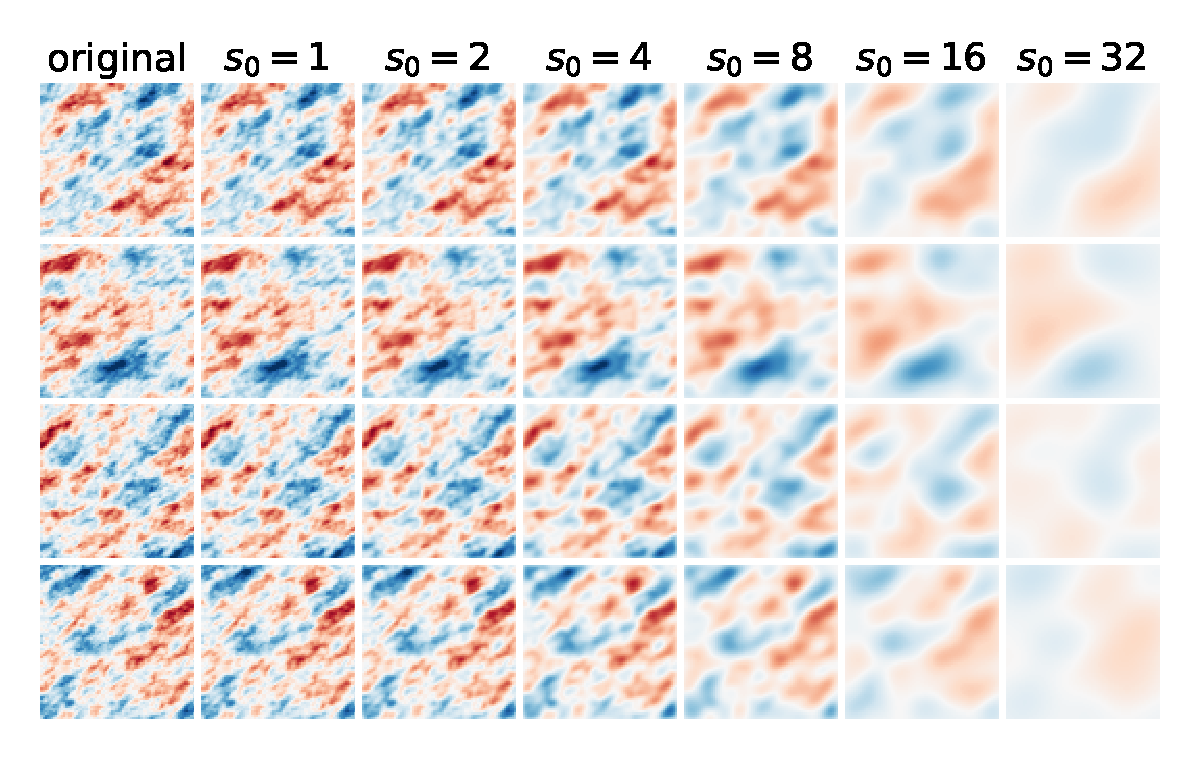
\includegraphics[width=\linewidth]{Figures/fake-seeing-nonp-thumbnails}\\
    (b)\\
    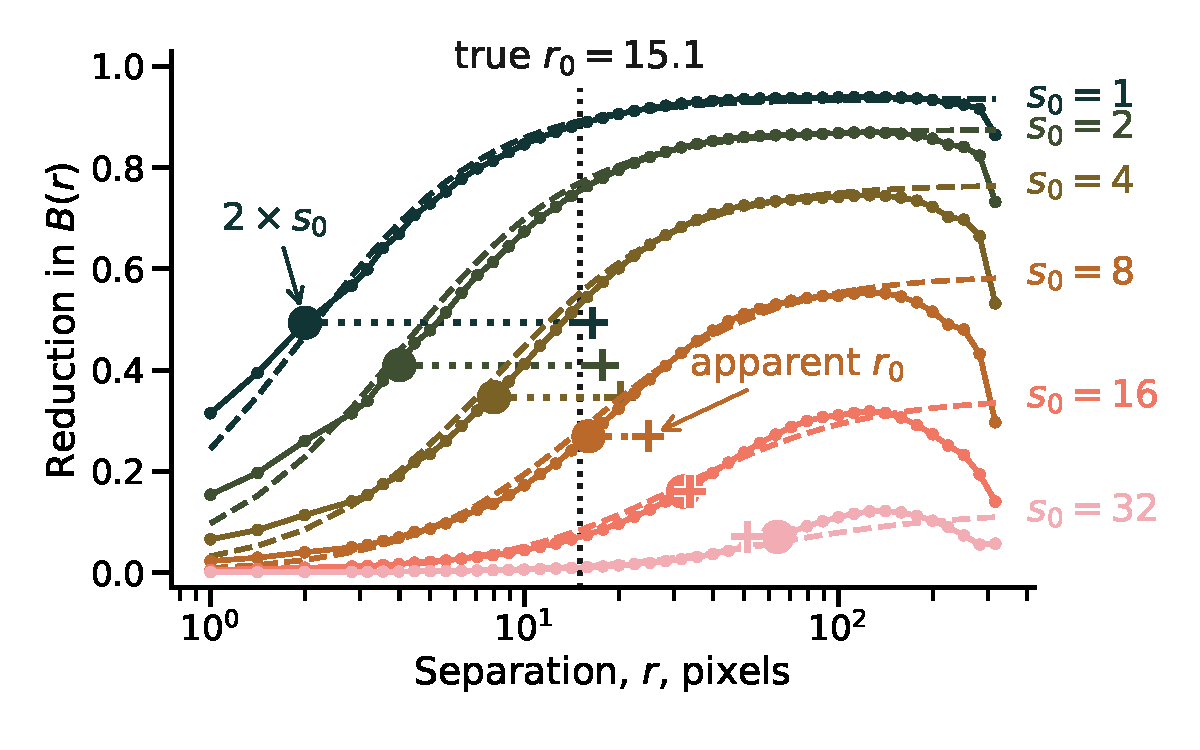
\includegraphics[width=\linewidth]{Figures/fake-seeing-nonp-reduction}
  \end{tabular}
  \caption{Effects of seeing on the structure function.
    (a)~Each row shows a different simulated random velocity field on a \(256^2\) grid
    (see text for details).
    The left column shows the original field,
    while the remaining columns show the effects of smoothing by a gaussian kernel
    with RMS width \(s_0\) from 1 to 32 pixels.
    The same color scale is used for all columns, ranging from \(-3\) to \(+3\) times
    the standard deviation of the unsmoothed map.
    (b)~Relative change in the second-order structure function due to the gaussian smoothing.
    Solid lines with symbols show the average over the 4 maps of
    \(B(r, s_0) / B(r, s_0 = 0)\) as a function of separation \(r\),
    with a separation of \(2 s_0\) indicated by a large filled circle on each curve.
    Dashed lines shows the empirical fit discussed in the text.
    The dotted line shows the correlation length of the original fields,
    while colored plus symbols show the apparent correlation length of the smoothed fields.
  }
  \label{fig:seeing-reduction}
\end{figure}


%%%%%%%%%%%%%%%%%%%%%%%%%%%%%%%%%%%%%%%%%%%%%%%%%%
%%%%%%%%%%%%%%%%%%%%% END %%%%%%%%%%%%%%%%%%%%%%%%
%%%%%%%%%%%%%%%%%%%%%%%%%%%%%%%%%%%%%%%%%%%%%%%%%%

% Don't change these lines
\bsp	% typesetting comment
\label{lastpage}
\end{document}

% End of mnras_template.tex
%%% Local Variables:
%%% mode: latex
%%% TeX-master: t
%%% End:
